%------------------------------------------------------------------------------
% Supporting information for Acta Crystallographica Section A, prepared with the
% IUCr LaTeX macro package (iucr.cls).  Compile with pdflatex.
%------------------------------------------------------------------------------
\documentclass[preprint,pdf]{iucr}          % DO NOT DELETE THIS LINE
\journalcode{A}

\usepackage{amsmath,amssymb}
\usepackage{booktabs}
\usepackage{array}
\usepackage{graphicx}

\newcommand{\Ang}{\text{\AA}}
\newcommand{\Gmet}{\mathbf{G}}
\newcommand{\Pop}{\mathbf{P}}
\newcommand{\Wop}{\mathbf{W}}
\newcommand{\Sw}{\mathcal{S}_\tau}
\newcommand{\Se}{\mathcal{S}_\eta}
\newcommand{\Cl}{\mathcal{C}}
\newcommand{\Lay}{\mathcal{N}}
\newcommand{\sym}{\operatorname{sym}}
\newcommand{\dist}{D}

\begin{document}

\title{Supporting information for \emph{The Selling closure: a complete operator set for reindexing, and the price of pseudo-symmetry}}
\shorttitle{The Selling closure: supporting information}
\cauthor{Petrus H.}{Zwart}{phzwart@lbl.gov}{}
\aff{Molecular Biophysics and Integrated Bioimaging Division, Lawrence Berkeley National Laboratory, 1 Cyclotron Road, Berkeley, CA 94720, \country{USA}}
\shortauthor{Zwart}
\maketitle

\renewcommand{\thesection}{S\arabic{section}}
\renewcommand{\thetable}{S\arabic{table}}
\renewcommand{\thefigure}{S\arabic{figure}}
\setcounter{table}{0}

All code is in \texttt{agentsg} (Zwart, 2026), version 0.5.0, \texttt{github.com/phzwart/agentsg}; the scripts named below are in its directory \texttt{manuscript/\allowbreak supplement/\allowbreak benchmark}, and the checks in the package \texttt{sellingproofs} (Section~S7). Table, section and equation numbers of the main text are cited as there. Conorm vectors are written in the slot order $da,db,dc,ab,ac,bc$ of the main text, and strains in per cent. Section~S7 lists, for every section, table and figure, the check that reproduces its numbers. Terms are those of the main text (Table~2): a \emph{step} is a Selling step, and at a zero conorm a boundary transformation; a \emph{face} is the set of conorm vectors with a given zero pattern, a boundary of the cone of reduced conorms; a \emph{difference-wall member} is a member of a widened set that is reachable from the reduced cell only through a non-member, across the wall where two small conorms are equal.

%==============================================================================
\section{Catalogues of shapes and specialisations}\label{app:catalogues}

\emph{Cell shapes.} Table~\ref{tab:shapes} lists the shapes of the ten sorts with more than one, each as the cell with the most right angles and no acute angle. The three shapes of a primitive monoclinic lattice are the three cell choices of \emph{International Tables} (Hahn, 2006, Section~2.2.16); the extra shapes of primitive orthorhombic, tetragonal and cubic lattices are monoclinic-looking cells with two right angles; C-centred orthorhombic has two primitive shapes; the boundary sorts of body-centred orthorhombic, C-centred monoclinic and triclinic have two or three cells with a single right angle each, for triclinic the known instability of the reduced cell when an angle is near $90^\circ$ (Andrews \emph{et al.}, 1980).

\begin{table}
\caption{The cell shapes of the sorts with more than one, for the cells named; each shape is given as the cell with the most right angles and all angles $\ge90^\circ$, shortest edges first when several qualify and $b$ unique for the monoclinic-looking ones, with the number $n$ of members (up to relabellings) that have it. Centred cells are given by their primitive cells; the boundary sorts are specified by their conorms in \Ang$^2$.}
\label{tab:shapes}
\begin{footnotesize}
\begin{tabular}{llrl}
\toprule
sort & lattice & $n$ & shape \\
\midrule
cP & $30$\,\Ang & 4 & $30$, $30$, $30$; $90$, $90$, $90$ \\
   &            & 12 & $30$, $30$, $42.4$; $90$, $135$, $90$ \\
tP & $30$, $30$, $50$\,\Ang & 4 & $30$, $30$, $50$; $90$, $90$, $90$ \\
   &            & 4 & $30$, $30$, $58.3$; $90$, $121.0$, $90$ \\
   &            & 8 & $30$, $50$, $42.4$; $90$, $135$, $90$ \\
oP & $30$, $40$, $55$\,\Ang & 4 & $30$, $40$, $55$; $90$, $90$, $90$ \\
   &            & 4 & $30$, $40$, $62.6$; $90$, $118.6$, $90$ \\
   &            & 4 & $30$, $55$, $50$; $90$, $126.9$, $90$ \\
   &            & 4 & $40$, $55$, $50$; $90$, $143.1$, $90$ \\
oS & C $30$, $40$, $50$\,\Ang & 2 & $25$, $50$, $25$; $90$, $106.3$, $90$ \\
   &            & 4 & $25$, $50$, $30$; $90$, $126.9$, $90$ \\
mP & $30$, $40$, $50$\,\Ang, $100^\circ$ & 2 & $30$, $40$, $50$; $90$, $100$, $90$ \\
   &            & 2 & $30$, $40$, $53.7$; $90$, $113.4$, $90$ \\
   &            & 2 & $50$, $40$, $53.7$; $90$, $146.6$, $90$ \\
oI (O3) & $900$, $1600$, $0$, $0$, $1600$, $900$ & 1 & $50$, $50$, $50$; $111.1$, $129.8$, $90$ \\
   &            & 2 & $42.4$, $50$, $50$; $90$, $115.1$, $115.1$ \\
mC (M2B) & $900$, $1600$, $2500$, $0$, $1600$, $900$ & 1 & $50$, $50$, $70.7$; $104.7$, $116.9$, $90$ \\
   &            & 1 & $50$, $50$, $65.6$; $105.9$, $105.9$, $90$ \\
mC (M3) & $2500$, $1600$, $0$, $0$, $1600$, $900$ & 1 & $50$, $50$, $64.0$; $120$, $90$, $111.1$ \\
   &            & 2 & $50$, $56.6$, $58.3$; $90$, $108.0$, $124.4$ \\
aP (A2) & $2500$, $400$, $1200$, $0$, $1600$, $900$ & 1 & $36.1$, $60.8$, $64.0$; $114.3$, $90$, $114.2$ \\
   &            & 1 & $36.1$, $56.6$, $64.0$; $116.2$, $90$, $101.3$ \\
aP (A3) & $2500$, $400$, $0$, $0$, $1600$, $900$ & 1 & $36.1$, $50$, $53.9$; $90$, $101.9$, $119.9$ \\
   &            & 1 & $44.7$, $50$, $53.9$; $90$, $99.6$, $135.7$ \\
   &            & 1 & $36.1$, $44.7$, $58.3$; $90$, $115.3$, $104.4$ \\
\bottomrule
\end{tabular}
\end{footnotesize}
\end{table}

\emph{Specialisations.} The conorms of any member, in any labelling, are integer combinations of the reduced cell's conorms, hence linear in the free parameters of the sort (the letters of Table~\ref{tab:sorts}). Imposing another sort's zeros and equalities on one member is a homogeneous linear system in those parameters, and a solution with non-negative parameters, a non-singular lattice and a resulting lattice of the target sort and no higher is a specialisation. Table~\ref{tab:special} lists the conditions of codimension one, on 36 pairs of sorts. Each is a parameter vanishing or two parameters becoming equal. The classical values appear: body-centred tetragonal is face-centred cubic at $c/a=\sqrt2$ and body-centred cubic at $c/a=1$; C-centred orthorhombic is hexagonal at $b=\sqrt3\,a$ and tetragonal at $b=a$; rhombohedral is cubic at $\alpha=60^\circ$, $90^\circ$ and $109.47^\circ$. The monoclinic conditions come in threes, one per shape: with unique axis $c$ and plane lattice $a,b$, the lattice is C-centred orthorhombic when $|a|=|b|$, $|a|=|a+b|$ or $|b|=|a+b|$, and primitive orthorhombic when $a\perp b$, $a\perp(a+b)$ or $b\perp(a+b)$ --- the textbook condition $a=c$ read in each of the three cell choices. The table also shows which sorts are one condition from a much higher symmetry: C-centred monoclinic from tetragonal, body-centred tetragonal and rhombohedral; the body-centred orthorhombic boundary sort from face-centred cubic; triclinic on a wall from C-centred monoclinic.

\begin{table}
\caption{All specialisations of codimension one between the 24 sorts. Conditions are on the letters of the sort's pattern in Table~\ref{tab:sorts}; ``shapes'' is the number of distinct cell shapes of the starting sort through which the conditions are reached, and the last column reads the condition in the cell of the conventional description where that is short.}
\label{tab:special}
\begin{footnotesize}
\begin{tabular}{llllp{4.6cm}}
\toprule
from & to & conditions & shapes & reading \\
\midrule
aP A1 & aP A2 & any letter $=0$ & 1 & a right angle appears \\
aP A2 & aP A3 & $v=0$ & 1 & a second right angle \\
aP A2 & mC M2A & $s=t$, $r=u$ & 1 & \\
aP A2 & mP M4 & $r,s,t$ or $u=0$ & 1 & \\
aP A3 & mC M3 & any two letters equal & 3 & one per shape \\
mP M4 & oP O5 & $r=0$, $s=0$, $t=0$ & 3 & $a\perp b$, $a\perp(a+b)$, $b\perp(a+b)$ \\
mP M4 & oS O4 & $s=t$, $r=t$, $r=s$ & 3 & $|a|=|b|$, $|a|=|a+b|$, $|b|=|a+b|$ \\
mC M1A & oF O1A & $r=t$ & 1 & \\
mC M1A & oI O2 & $u=0$ & 1 & \\
mC M1A & oS O4 & $r=0$, $t=0$ & 1 & \\
mC M1B & mC M2B & $t=0$, $u=0$ & 1 & boundary sort \\
mC M1B & mC M3 & $r=0$, $s=0$ & 1 & boundary sort \\
mC M1B & oF O1A & $r=s$ & 1 & \\
mC M1B & oI O1B & $t=u$ & 1 & \\
mC M2A & oI O2 & $r=t$ & 1 & \\
mC M2B & oI O3 & $t=0$ & 1 & \\
mC M2B & tI T2 & $r=s$ & 1 & one step to tI \\
mC M2B & tP T5 & $r=0$, $s=0$ & 1 & one step to tP \\
mC M3 & oI O3 & $r=t$ & 1 & \\
mC M3 & hR R3 & $r=s$, $s=t$ & 1 & one step to hR \\
oP O5 & tP T5 & $r=s$, $r=t$, $s=t$ & 1 & $a=b$, $a=c$, $b=c$ \\
oS O4 & tP T5 & $r=0$ & 1 & $b=a$ \\
oS O4 & hP H4 & $r=s$ & 1 & $b=\sqrt3\,a$ \\
oI O1B & oI O3 & $r,s$ or $t=0$ & 1 & boundary sort \\
oI O1B & tI T1 & $r=s$, $r=t$, $s=t$ & 1 & two edges equal \\
oI O2 & tI T2 & $r=s$ & 1 & \\
oI O3 & cF C3 & $r=s$ & 1 & one step to cF \\
oF O1A & tI T1 & $s=t$ & 1 & \\
oF O1A & tI T2 & $s=0$, $t=0$ & 1 & \\
tP T5 & cP C5 & $r=s$ & 1 & $c=a$ \\
tI T1 & cI C1 & $r=s$ & 1 & $c/a=1$ \\
tI T1 & cF C3 & $s=0$ & 1 & $c/a=\sqrt2$ from below \\
tI T2 & cF C3 & $s=0$ & 1 & $c/a=\sqrt2$ from above \\
hR R1 & cP C5 & $r=0$ & 1 & $\alpha=90^\circ$ \\
hR R1 & cI C1 & $r=s$ & 1 & $\alpha=109.47^\circ$ \\
hR R3 & cF C3 & $r=s$ & 1 & $\alpha=60^\circ$ \\
\bottomrule
\end{tabular}
\end{footnotesize}
\end{table}

%==============================================================================
\section{The benchmark, the comparisons and the walks}\label{si:bench}

\emph{The benchmark.} The directory \texttt{manuscript/\allowbreak supplement/\allowbreak benchmark} of the repository holds 780 measured cells with exact references and true operators, in five families: 75 cells measured in a different shape of the same lattice; 660 lattices placed $0.5$ to $8$ times the error from a condition of Table~\ref{tab:special}; 20 cells whose only reduced superbase is a difference-wall member; 16 needles and plates with angular errors; 9 cells of the boundary sorts. Each case carries its Niggli cell. The errors are isotropic in the metric tensor, of median strain $0.1\%$. A case counts as found when the true proper operator itself is among the candidates. \texttt{evaluate\_strain.py} scores the closure and the $\{-1,0,1\}$ search at the band and at three times each case's error (\texttt{results\_strain.txt}); \texttt{evaluate.py --niggli} tallies the Niggli cells by family and sort (\texttt{results\_niggli.txt}). The measured Niggli cell is a different cell from the reference's in 45 cases (O1B 23, O3 12, M1B 6, one each at M2B, M3, R3 and T2; 14 of them a change between type~I and type~II), and the same cell in another basis in 125 (O1B 25, M1A 15, O1A 15, T1 15, M1B 13, O4 9, O2 7, R1 7, M2A 6, T2 6, O3 5, A2 1, A3 1).

{\sloppy \emph{The comparisons.} \texttt{compare\_methods.py} runs the searches of Table~\ref{tab:searches} on the benchmark (\texttt{results\_compare.txt}) and, with \texttt{--stress}, on the stress family (\texttt{results\_stress.txt}): 60 references drawn from the benchmark, each with independent traceless errors on the reference and the new cell, scaled so that the true operator's price is $t$ times the band, $t=0.5$, $0.9$, $1.1$ and $1.5$, and a random proper reindexing with entries in $\{-2,\dots,2\}$. Each method's candidates are made proper, priced by the geodesic distance after the best scale, and kept within the band; at $t=1.1$ and $1.5$ no method found the true operator, as by construction none should. \texttt{window\_failures.py} builds the window family (\texttt{results\_window\_failures.txt}): 300 lattices of the sorts M4, O4, H4, O5, T5 and C5 with random parameters, each measured twice with an error of $0.1$ to $2\%$, the new cell in a random proper basis and the reference given as its Niggli cell, classified by the Niggli type of the reference and by the kind of face (with an exact reference in the labelling of the sort's pattern the zeros never sit on $d$ and no window fails); the same 300 lattices, drawn again, with the reference in a random proper basis; and 60 lattices on random two- and three-zero faces whose closure has a member needing an entry of $3$, measured in that member. \texttt{coset\_rank.py} groups the closure's candidates by the exact symmetries of the underlying lattice (\texttt{results\_coset.txt}). \texttt{niggli\_types.py} reduces near-monoclinic cells from their Niggli cells and records where the near-zero conorms land (\texttt{results\_niggli\_types.txt}). \texttt{face\_labellings.py} gives, for every face, the largest entry of the operators out of the reduced cell as reduction returns it and in its best labelling (\texttt{results\_face\_labellings.txt}). \texttt{lookup\_benchmark.py} runs the lookup of $\mathcal U$ on the benchmark and the stress family and counts the references whose $r_1$ does not certify it (\texttt{results\_lookup.txt}). \texttt{benchmark\_misses.py} lists the benchmark cases that the $\{-1,0,1\}$ window and the pipeline miss (\texttt{results\_benchmark\_misses.txt}). \texttt{niggli\_presentation.py} reduces measured near-oP cells from their Niggli form and from random bases and records where the near-zero conorms land (\texttt{results\_niggli\_presentation.txt}). \texttt{lookup\_plate\_case.py} builds the plate case in which an uncertified lookup misses an operator (\texttt{results\_lookup\_plate\_case.txt}). \texttt{export\_universal\_operators.py} writes $\mathcal U$ as column operators with their determinants (\texttt{universal\_operators\_columns.json}). \texttt{adjacency\_radii.py} computes $r_1$ for the benchmark references and for 2000 PDB cells drawn at random, and times the widening and the reindexing (\texttt{results\_adjacency\_radii.txt}).\par}

{\sloppy\emph{The PDB.} \texttt{pdb\_nonisomorphism.py} measures the price between entries of one crystal form (\texttt{results\_pdb\_nonisomorphism.txt}). \texttt{pdb\_lepage.py} runs the cctbx lattice-symmetry analysis at $3^\circ$ on every entry and prices the pseudo-symmetries (\texttt{pdb\_lepage.jsonl}, \texttt{results\_pdb\_lepage.txt}); \texttt{pdb\_pricing\_summary.py} gives the transitions and the fractions within the non-isomorphism band (\texttt{results\_pdb\_pricing.txt}). \texttt{pdb\_band\_controls.py} varies the cut between crystal forms, drops identical cells, weights deposition blocks equally, splits the band by Bravais type, and counts on 3000 same-form pairs how often a wrong class is cheaper than the identity's (\texttt{results\_pdb\_band\_controls.txt}). \texttt{pdb\_lepage\_null.py} compares the Le Page rate of real cells with that of cells whose parameters are shuffled within a space group (\texttt{results\_pdb\_lepage\_null.txt}). Table~\ref{tab:pdbsort} lists the prices by the Delone sort of the Le Page lattice and Table~\ref{tab:pdbtrans} by transition from the reported type.\par}

\emph{Walks.} Table~\ref{tab:walks} compares four walks on the measured metric, with a band $\tau$ on the conorms, and the construction of Section~S4 against brute force.

\begin{table}
\caption{Four walks on the measured metric, and the construction of Section~S4, against brute force on 80 cells with zero conorms at awkward positions (orthorhombic, cubic, plate, monoclinic and hexagonal zero patterns), with a band $\tau$ on the conorms at $0.1$ and $0.5$ of $\lambda_1/32$.}
\label{tab:walks}
\begin{tabular}{lc}
\toprule
procedure & cells with a wrong set \\
\midrule
step wherever $|p|\le\tau$, keep only cells within the band & 13 \\
step wherever $|p|\le\tau$, filter at the end & 13 \\
step wherever $|p|\le2\tau$, keep only cells within the band & 13 \\
step wherever $|p|\le2\tau$, filter at the end & 2 \\
idealise at $4\tau$, enumerate the exact closure, filter & 0 \\
\bottomrule
\end{tabular}
\end{table}

%==============================================================================
\section{The operators alone}\label{app:operators}

The closure can be described without any lattice. An operator $\Wop$, written as the new basis in the coordinates of the reduced cell, acts on the six conorms by a fixed integer $6\times6$ matrix $\mathbf A_{\Wop}$, since every conorm of $\Wop F_0$ is an integer combination of the conorms of $F_0$. The reduced cells are the points of the orthant $\{p\ge0\}$ in conorm space. Selling (1874) showed that every lattice has a conorm vector in this orthant, unique up to the 48 relabellings except on the faces (Delaunay, 1933; Conway \& Sloane, 1992), and the closure of a lattice is the set of points of its orbit that lie in the orthant: one in the interior, several on the faces. So $\Wop$ is an operator of the closure of every lattice on the face of $Z$ exactly when $\mathbf A_{\Wop}$ maps the face $\{p\ge0,\ p_Z=0\}$ into the orthant, a sign condition on the entries of $\mathbf A_{\Wop}$ and nothing else.

Enumerating integer matrices with entries in $[-2,2]$ under that condition, over all 38 faces, and closing the result under relabelling at both ends, gives a set $\mathcal U$ of $6096=48\times127$ integer matrices with entries in $\{-3,\dots,3\}$; per face there are $48\times1$, $2$, $3$, $6$ and $16$ matrices for no zero, one zero, two zeros on disjoint pairs, two zeros sharing a vector and three zeros. Both placements of three zeros, the triangle and the path, were enumerated; they describe the same lattices read from an orthogonal cell or from a cell with a face diagonal, each has 16 members, and no relabelling carries one placement into the other. $\mathcal U$ is closed under inversion, and every element has a labelling whose basis vectors have entries in $[-2,2]$. That $\mathcal U$ contains every operator between two reduced cells of one lattice, whatever the lattice, does not rest on that window: Lemma~A2 of the main text confines the members of every closure to superbase coordinates $s+2k$ with $|k_i|\le3$ relative to a reduced cell, and the enumeration of that whole window, over all 38 faces, finds only members that lie in $\mathcal U$ in each of their 48 labellings. In the basis of the reduced cell their entries are in $\{-1,0,1\}$ when the zero conorms avoid $d$, and up to $3$ otherwise (Table~4 of the main text). Up to relabelling at both ends $\mathcal U$ has nine kinds of element, of step length $0$ to $4$ (Table~\ref{tab:kinds}).

\begin{table}
\caption{The nine kinds of operator between Selling-reduced cells, up to relabelling at both ends; ``matrices'' counts the integer matrices of the kind in $\mathcal U$, ``steps'' its length as a word of steps, and the last column the zero patterns in whose closures it occurs.}
\label{tab:kinds}
\begin{footnotesize}
\begin{tabular}{rrrl}
\toprule
kind & matrices & steps & occurs with \\
\midrule
1 & 48 & 0 & every pattern (the relabellings) \\
2 & 288 & 1 & every pattern with a zero \\
3 & 1152 & 2 & two zeros sharing a vector; three zeros \\
4 & 1152 & 3 & three zeros \\
5 & 1152 & 3 & three zeros \\
6 & 576 & 3 & two zeros sharing a vector; three zeros \\
7 & 576 & 4 & three zeros \\
8 & 576 & 4 & three zeros \\
9 & 576 & 4 & three zeros \\
\bottomrule
\end{tabular}
\end{footnotesize}
\end{table}

\emph{Why four.} For a lattice with $a\perp b\perp c$ the sixteen members are four orthogonal superbases, differing by the sign of one axis, and twelve with a face diagonal. A step from an orthogonal cell always gives a cell with a face diagonal, so changing the sign of one axis takes three steps, out, across and in, and the diagonal cells attached only to the far orthogonal cell take one more: from $(a,b,c)$ the members lie at step distances $0,1,2,3,4$ in numbers $1,3,6,3,3$, and four is the diameter of the largest face.

%==============================================================================
\section{A band on the conorms}\label{app:tau}

The simplest widening of the closure is an absolute band $\tau$ in \Ang$^2$ on the conorms,
\begin{equation}
\Sw(\Gmet)=\bigl\{\,F\;:\;\text{all six conorms of }F\text{ under }\Gmet\text{ are}\ \ge-\tau\,\bigr\},
\label{eq:deftau}
\end{equation}
Selling reduction with its boundary moved from $0$ to $-\tau$. This is an $L^\infty$ band on the conorms, a different norm from the strain of the main text; the two are comparable only for cells whose edges are similar in length. It can be computed by idealising: set every conorm of the reduced superbase $F_0$ that is at most $4\tau$ to zero, enumerate the exact closure of the idealised lattice $\Lambda^*$, and keep the members whose conorms under the measured metric are all at least $-\tau$. The construction is exact when $\lambda_1$, the squared length of the shortest lattice vector, exceeds $32\tau$ (Theorem~S4.5), a ratio independent of the scale of the cell: for an isotropic cell it allows an angular error of about $1.8^\circ$. It fails for anisotropic cells, where the band must cover the conorms between the long vectors: on the 16 needles and plates of the benchmark it declined 8. On monoclinic, hexagonal, orthorhombic, cubic and plate lattices (two zero conorms sharing a vector, or three forming a triangle), with zero conorms placed at random, it agreed with brute force over bases with entries in $[-2,2]$ at every band from $\lambda_1/32$ to $\lambda_1/6$ in which the idealised lattice existed; beyond the hypothesis that window is not proved to hold the whole set. On dense grids of two small conorms, idealising at $\tau$ instead of $4\tau$ was already exact at the monoclinic and hexagonal corners, and missed members at the orthorhombic and cubic corners exactly when $z\le\tau<y\le z+\tau$ for the two small conorms $z\le y$; idealising at $2\tau$ was exact there. For the worked cell at $\tau=20$\,\Ang$^2$, within the hypothesis, it returns the six members of the ring. A new cell constructed so that its only reduced superbase is a difference-wall member of an orthorhombic corner was matched against two stored sets of the reference: the complete set offers three candidates and their negatives; a set built by idealising only at the band has lost the third, $\pm\mathbf I$, the true operator.

\emph{Bands per slot.} A band that scales with the vectors of each superbase, $p_{ij}(F)\ge-\sigma|u_i||u_j|$ on every slot of $F$ (all pairwise angles at least $90^\circ-\arcsin\sigma$), is the natural angular form of the $L^\infty$ band, but the same construction applied with each slot of $F_0$ idealised against its own band is not exact. On the needle $5.58\times5.21\times131.97$\,\Ang, $\gamma=91.12^\circ$, at $\lambda_1/(\sigma l_al_c)=33$ and $40$, it returns 6 superbases where brute force finds 12: the conorm $ab$ survives idealisation because its own band is small, while the members built on $a+c$ carry the same dot product on a slot whose band is about 25 times larger. Idealising until the zeroed slots are consistent across the members of the closure repairs this, and on 60 random needles, plates, isotropic and monoclinic cells, each at four bands (240 cases) it is never wrong (exact in 124, refused in 116), while the single-pass construction is wrong in 9 (z57).

For a superbase $F$ and two metrics, $\kappa_F(\Gmet,\Gmet')$ is the largest change among $F$'s six conorms.

\emph{Proposition S4.1 (characterisation superbase by superbase).} $\Sw(\Gmet)=\{F:F\in\Cl(\Gmet')\text{ for some }\Gmet'\text{ with }\kappa_F(\Gmet,\Gmet')\le\tau\}$. \emph{Proof.} ($\supseteq$) If $F$ is obtuse for $\Gmet'$ and $\kappa_F\le\tau$, every conorm of $F$ under $\Gmet$ is at least $-\tau$. ($\subseteq$) The metric whose conorms in the basis of $F$ are $\max(p_{ij},0)$ exceeds $\Gmet$ by a positive semidefinite term, so it is positive definite and $F$ is obtuse for it.\hfill$\square$

\emph{Lemma S4.2 (class gap).} Let $\Lambda^*$ be obtained from $F_0$ by setting its conorms $\le\theta$ to zero, be positive definite, and let $m^*$ be the smallest conorm of $F_0$ above $\theta$. A superbase not obtuse for $\Lambda^*$ has $e_c\ge4m^*$ in some class, the excess taken for $\Lambda^*$. \emph{Proof.} In the basis of $F_0$, Lemma~A1 of the main text gives $e_c(F)=4\sum p^0_{ij}\gamma_{ij}$, and the excess for $\Lambda^*$ is the same sum over the slots above $\theta$. If those terms vanish in all seven classes, $F$ is obtuse for $\Lambda^*$; otherwise some $\gamma_{ij}\ge1$ multiplies a $p^0_{ij}\ge m^*$.\hfill$\square$

\emph{Lemma S4.3 (small excess in the band).} If $\lambda_1>32\tau$ and every conorm of $F$ is at least $-\tau$, then $e_c(F)\le16\tau$ in every class. \emph{Proof.} Call a slot large if $p_{ij}>8\tau$, and let $N$ be the negative slots. The large slots connect the four vectors, since otherwise a split crossed only by slots with $p_{ij}\le8\tau$ has a partial sum of squared length at most $32\tau<\lambda_1$. Lemma~A1 in the basis of $F$ gives $0\le e_c(F)=4\sum_N|p_{ij}|\gamma_{ij}-4\sum_{p_{ij}>0}p_{ij}\gamma_{ij}$, so $\sum_{\rm large}p\gamma\le\tau\sum_N\gamma$. If a large $\gamma$ were positive, Lemma~S4.4(ii) would give $8\tau\sum_{\rm large}\gamma<\tau\sum_N\gamma\le8\tau\sum_{\rm large}\gamma$; so the large $\gamma$ vanish, and Lemma~S4.4(i) gives $e_c\le4\tau\cdot4$.\hfill$\square$

\emph{Lemma S4.4 (two constants on four points).} Let $L$ be a set of slots connecting the four vectors and $N$ disjoint from $L$. (i) If $\gamma_{ij}=0$ on $L$, then $\sum_N\gamma_{ij}\le4$. (ii) If $\sum_L\gamma_{ij}>0$, then $\sum_N\gamma_{ij}\le8\sum_L\gamma_{ij}$. Both bounds are attained. \emph{Proof.} In (i) $|\Delta k|\le1$ on $L$, so all $|k_i|\le3$, and the maximum is a finite enumeration over the 38 connected slot sets, the sets $N$ and the 14 partial sums. In (ii) the ratio is enumerated for $|k_i|\le15$; beyond, some $|k_i|\ge16$, and since $L$ connects the four vertices with $k_0=0$, $Q=\sum_L\Delta k^2\ge16^2/3>75$. For each pattern $(L,N)$ let $\rho_{L,N}$ be the largest generalised eigenvalue of the quadratic form $\sum_N\Delta k^2$ against $\sum_L\Delta k^2$; the largest over all pairs $(L,N)$ is $3+2\sqrt2$. Then $\sum_N\gamma\le\rho_{L,N}Q+\sqrt{|N|\rho_{L,N}Q}$ and $\sum_L\gamma\ge Q-\sqrt{|L|Q}$, and the ratio of these bounds, $(\rho_{L,N}\sqrt Q+\sqrt{|N|\rho_{L,N}})/(\sqrt Q-\sqrt{|L|})$, decreases in $Q$, so it suffices to check it at $Q=75$ for each pattern with its own $\rho_{L,N}$, where it is below $8$ in every case; with the uniform value $3+2\sqrt2$ it would not be. The lemma is computer-assisted. Equality in (ii): $L=\{01,02,13\}$, $N=\{03,12,23\}$, $s=(0,0,1,1)$.\hfill$\square$

\emph{Theorem S4.5.} Let $F_0$ be obtuse for $\Gmet$, $\lambda_1>32\tau$, and $\Lambda^*$ obtained by setting every conorm of $F_0$ that is at most $4\tau$ to zero. Then $\Lambda^*$ is positive definite and $\Sw(\Gmet)=\{F\in\Cl(\Lambda^*):p_{ij}(F;\Gmet)\ge-\tau\}$. \emph{Proof.} If the slots of $F_0$ above $4\tau$ did not connect the four vectors, some partial sum would have squared length at most $16\tau<\lambda_1$. The inclusion $\supseteq$ is the definition. For $F\in\Sw(\Gmet)$, Lemma~S4.3 gives $e_c(F;\Gmet)\le16\tau$; the excess for $\Lambda^*$ is the same sum with the zeroed slots dropped, so $e_c(F;\Lambda^*)\le16\tau<4m^*$, and Lemma~S4.2 makes $F$ obtuse for $\Lambda^*$.\hfill$\square$ The operators from $F_0$ to the members of $\Cl(\Lambda^*)$ are integer matrices independent of the metric, so one enumeration serves every band up to the one idealised at.

\emph{Lemma S4.6 (nesting).} If $Z'\subseteq Z$ are sets of conorms of $F_0$ set to zero, every member of the closure for $Z'$ is a member of the closure for $Z$. \emph{Proof.} The members for $Z'$ are reached from $F_0$ by words of steps, each at a slot that is zero at that point of the word (Lemma~A3 of the main text); a step at a slot zero for both lattices acts on both conorm vectors as the same transposition of two slots, so after each step the superbase is obtuse for both and the next step is again at a slot zero for both.\hfill$\square$

\emph{Proposition S4.7 (reindexing guarantee in the reference basis).} Let $\Gmet_N'$ be the new cell's metric written in the reference's reduced basis, $\|\Gmet_N'-\Gmet_R\|_F\le\xi<\nu_{\min}$ with $\nu_{\min}$ the smallest eigenvalue of $\Gmet_R$, let $F_N$ be its reduced superbase with basis vectors of summed squared length $V$, and let $\tau\ge\sqrt2\,\xi\,V/(\nu_{\min}-\xi)$ with $\lambda_1(\Gmet_R)>32\tau$. Then $F_N$, with its true integer coefficients in the reference basis, is a member of $\Sw(\Gmet_R)$, and pairing it with the new cell's reduced superbase proposes the true operator. \emph{Proof.} With $u_1,u_2,u_3$ the coordinate vectors of $F_N$'s basis in the reference basis and $\Delta=\Gmet_N'-\Gmet_R$, $\sum|u_i|^2\le V/(\nu_{\min}-\xi)$; in $F_N$'s own basis the error has Frobenius norm at most $\sum|u_i|^2\,\xi$, and every conorm shift is at most $\sqrt2$ times that norm. The conorms of $F_N$ under $\Gmet_N'$ are non-negative, so under $\Gmet_R$ they are at least $-\tau$, and Theorem~S4.5 applies.\hfill$\square$ For fifteen references near the zero conorms of monoclinic, hexagonal, orthorhombic, cubic and plate lattices, each with twelve new cells carrying a random metric error and a random reindexing, the true operator was among the candidates in 180 of 180 cases at the band given by the coverage bound below, between $0$ and $8\xi$ for these references; the guarantee of Proposition~S4.7 is conservative, asking for a median $13\xi$ (from $4.3\xi$ to $75\xi$).

\emph{From a metric error to a band.} A metric error $\Delta\Gmet$ shifts the conorm of a member with coordinate vectors $u_i,u_j$ by $-u_i^{\mathsf T}\Delta\Gmet\,u_j$, at most $c_{ij}\xi$ with $c_{ij}=\|\sym(u_iu_j^{\mathsf T})\|_F$; every member survives every error of norm $\xi$ exactly when $\tau\ge\tau_{\rm cov}=\max(c_{ij}\xi-p_{ij})$, read off the stored closure. The largest constant on zero conorms is $\sqrt2$ with one zero, $\sqrt5$ with two, and $2\sqrt3$ in six of the sixteen labelled cuboid bases, so $\tau=3\xi$ is not a worst-case guarantee in every basis. These basis-dependent constants are what the strain norm removes.

%==============================================================================
\section{Further tables}

\begin{table}
\caption{The seven sample cells of BLDConograph (Oishi-Tomiyasu, 2024): the program's Bravais type and its minimal distance to that type (\Ang$^2$), and the same divided by the mean squared edge (\%); the Bravais types of the sort spectrum in increasing strain distance (\%), aP omitted, up to and including the program's type; and the next type with its distance. For all seven cells $r_1$ reaches the cap, so ``$>25$'' is a lower bound on the distance as well as the outcome of the minimum over the bases of $\mathcal U$. A band of $7.4\%$ selects the program's type in all seven; the largest ratio between consecutive distances follows it in six, and for the alumina cell lies between mC and hR.}
\label{tab:conograph}
\begin{footnotesize}
\begin{tabular}{llrrp{4.6cm}l}
\toprule
sample & type & \Ang$^2$ & \% & types up to the program's (strain \%) & next \\
\midrule
HERMES\_Sr327\_250K & tI & 0.57 & 1.24 & mC 0.31, oI 0.74, oF 0.83, tI 0.84 & mP $>25$ \\
1339prbasrcuo\_bs1 & tP & 0.056 & 0.10 & mP 0.11, mC 0.14, oS 0.17, oP 0.18, tP 0.22 & oF $>25$ \\
sample3 & cI & 2.07 & 0.78 & mC 0.23, hR 0.39, oF 0.39, oI 0.49, tI 0.49, cI 0.58 & cF $>25$ \\
CeO2\_matsushita & cF & 0.084 & 0.61 & mC 0.09, oI 0.17, oF 0.17, tI 0.18, hR 0.26, cF 0.30 & cI $>25$ \\
M402-pf-119673 & hP & 20.5 & 5.28 & mC 0.99, mP 2.24, oS 2.37, hP 2.94 & oI $>25$ \\
Acrinol-B-D8CuKa1 & mC & 0.72 & 0.35 & mC 0.31 & oF 20.6 \\
Alumina676 & hR & 1.93 & 8.11 & mC 0.43, hR 3.58 & oI 14.9 \\
\bottomrule
\end{tabular}
\end{footnotesize}
\end{table}

\begin{table}
\caption{The widened closure of the measured worked cell. Each row is a member, named by a word in the steps of Table~1 of the main text from the reduced cell $e$ (the empty word); the six numbers are its conorms under the measured metric, in \Ang$^2$; ``depth'' is the strain at which it enters, in \%. At a strain of $7.7\%$, the widening for the default band, all sixteen are members.}
\label{tab:filter}
\begin{footnotesize}
\begin{tabular}{lrrrrrrr}
\toprule
word & $da$ & $db$ & $dc$ & $ab$ & $ac$ & $bc$ & depth \\
\midrule
$e$ & 49.5 & 1588.9 & 2444.7 & 4.2 & 847.5 & 4.5 & 0 \\
$bc$ & 45.0 & 8.7 & 2449.3 & 1593.4 & 852.0 & $-4.5$ & 0.28 \\
$ab$ & 851.7 & 1593.1 & 2440.6 & $-4.2$ & 53.7 & 8.7 & 0.49 \\
$bc.db$ & 2458.0 & $-8.7$ & 53.7 & 1602.1 & 843.3 & 4.2 & 0.62 \\
$ab.bc$ & 842.9 & 4.5 & 2449.3 & 1601.8 & 62.5 & $-8.7$ & 0.78 \\
$ab.bc.db$ & 2453.8 & $-4.5$ & 847.5 & 1606.3 & 57.9 & $-4.2$ & 0.78 \\
\midrule
$da$ & $-49.5$ & 2494.3 & 1638.4 & 53.7 & 897.0 & $-45.0$ & 3.76 \\
$ab.bc.ac$ & 1664.2 & $-57.9$ & 2511.7 & 905.4 & $-62.5$ & 53.7 & 4.56 \\
$da.ab$ & 950.7 & 2548.0 & 1584.7 & $-53.7$ & 4.2 & 8.7 & 5.06 \\
$da.ab.ac$ & $-49.5$ & 2543.8 & 1588.9 & 954.9 & $-4.2$ & 12.9 & 5.08 \\
$ab.ac$ & 49.5 & 1539.3 & 2494.3 & 905.4 & $-53.7$ & 62.5 & 5.08 \\
$da.ab.bc$ & 942.0 & $-45.0$ & 1593.4 & 2556.7 & 12.9 & $-8.7$ & 5.09 \\
$bc.db.dc$ & 45.0 & 2511.7 & $-53.7$ & 1548.4 & 897.0 & 57.9 & 5.09 \\
$ab.ac.bc.ac$ & 1610.5 & 959.1 & 2565.5 & $-4.2$ & $-8.7$ & $-53.7$ & 5.11 \\
$da.ab.bc.ac$ & 2569.6 & $-57.9$ & 1606.3 & 954.9 & $-12.9$ & 4.2 & 5.11 \\
$ab.ac.bc$ & $-12.9$ & 967.8 & 2556.7 & 1601.8 & 8.7 & $-62.5$ & 5.11 \\
\bottomrule
\end{tabular}
\end{footnotesize}
\end{table}

\begin{table}
\caption{The sort patterns of Andrews \& Bernstein (2023), in the $S^6$ slot order $bc,ac,ab,ad,bd,cd$, and the same patterns in the slot order $da,db,dc,ab,ac,bc$ of Table~\ref{tab:sorts}. The representative used here is their pattern read in the other order, with the sign of the Selling parameters reversed; no reflection is applied. Which zeros a pattern has also fixes the kind of face: for the three-zero sorts C5, T5 and O5 the zeros are $ab$, $ac$ and $bc$, a triangle on $a$, $b$, $c$, and the same lattices also have reduced cells whose zeros form a path.}
\label{tab:corr}
\begin{footnotesize}
\begin{tabular}{lll@{\hspace{2em}}lll}
\toprule
sort & $S^6$ order & this paper & sort & $S^6$ order & this paper \\
\midrule
C1 & rrrrrr & rrrrrr & O2 & rs0srt & srt0sr \\
C3 & rr0rr0 & rr00rr & O3 & rs0rs0 & rs00sr \\
C5 & 000rrr & rrr000 & O4 & 00rsst & sstr00 \\
H4 & 00rrrs & rrsr00 & O5 & 000rst & rst000 \\
T1 & rrsrrs & rrssrr & M1A & rrsttu & ttusrr \\
T2 & rr0rrs & rrs0rr & M1B & rstrsu & rsutsr \\
T5 & 000rrs & rrs000 & M2A & rs0stu & stu0sr \\
R1 & rrrsss & sssrrr & M2B & rs0rst & rst0sr \\
R3 & rr0sr0 & sr00rr & M3 & rs0ts0 & ts00sr \\
O1A & rrsrrt & rrtsrr & M4 & 00rstu & stur00 \\
O1B & rstrst & rsttsr & A1 & rstuvw & uvwtsr \\
 & & & A2 & rs0tuv & tuv0sr \\
 & & & A3 & rs0tu0 & tu00sr \\
\bottomrule
\end{tabular}
\end{footnotesize}
\end{table}

\begin{table}
\caption{Pseudo-symmetric PDB entries (Le Page lattice above the reported type at $3^\circ$) by the Delone sort of the Le Page lattice, operators of the reported lattice's own holohedry excluded, entries with an exact higher lattice included (their smallest price is $0$): number of entries, and the 10th/50th/90th percentiles of the largest obliquity $\delta$ (degrees) and of the largest and smallest price (\%) among the pseudo-symmetry operators of each entry. Sorts with no entries are omitted. The transitions from the reported type are in Table~\ref{tab:pdbtrans}. From \texttt{results\_pdb\_lepage.txt}.}
\label{tab:pdbsort}
\begin{footnotesize}
\begin{tabular}{llrccc}
\toprule
sort & type & entries & $\delta$ ($^\circ$) & largest price (\%) & smallest price (\%) \\
\midrule
C1 & cI & 593 & 0.14/1.64/2.73 & 0.69/8.10/13.58 & 0.32/7.13/13.18 \\
C3 & cF & 562 & 0.19/1.72/2.76 & 0.95/8.51/13.61 & 0.50/7.68/13.41 \\
C5 & cP & 1\,349 & 0.29/1.70/2.72 & 1.43/8.40/13.45 & 0.47/5.52/12.59 \\
H4 & hP & 2\,008 & 0.08/1.40/2.70 & 0.40/6.91/13.32 & 0.11/4.03/12.70 \\
T1 & tI & 1\,376 & 0.06/1.32/2.67 & 0.28/6.60/13.33 & 0.17/5.55/12.60 \\
T2 & tI & 330 & 0.05/1.48/2.69 & 0.24/7.30/13.43 & 0.11/4.98/12.44 \\
T5 & tP & 14\,816 & 0.22/1.47/2.69 & 1.07/7.27/13.43 & 0.70/6.56/12.98 \\
R1 & hR & 96 & 0.04/1.55/2.76 & 0.22/7.64/13.78 & 0.13/2.98/13.13 \\
R3 & hR & 393 & 0.07/1.82/2.81 & 0.37/9.09/13.86 & 0.29/7.64/13.72 \\
O1A & oF & 1\,126 & 0.23/1.51/2.70 & 1.12/7.45/13.33 & 1.02/7.05/13.17 \\
O1B & oI & 331 & 0.10/1.58/2.78 & 0.49/7.80/13.73 & 0.36/7.63/13.73 \\
O2 & oI & 1\,078 & 0.14/1.40/2.73 & 0.70/6.92/13.50 & 0.48/6.33/13.36 \\
O4 & oS & 11\,679 & 0.14/1.49/2.74 & 0.67/7.36/13.56 & 0.62/7.15/13.51 \\
O5 & oP & 4\,760 & 0.03/1.08/2.59 & 0.17/5.33/12.79 & 0.15/5.13/12.69 \\
M1A & mC & 867 & 0.72/2.09/2.83 & 3.53/10.33/13.98 & 3.53/10.33/13.98 \\
M1B & mC & 398 & 0.12/1.80/2.72 & 0.57/8.91/13.41 & 0.57/8.91/13.41 \\
M2A & mC & 854 & 0.13/1.75/2.77 & 0.66/8.64/13.66 & 0.66/8.64/13.66 \\
M2B & mC & 2 & 0.61/0.95/1.29 & 3.02/4.70/6.38 & 3.02/4.70/6.38 \\
M3 & mC & 1 & 2.39/2.39/2.39 & 11.80/11.80/11.80 & 11.80/11.80/11.80 \\
M4 & mP & 582 & 0.10/1.40/2.65 & 0.47/6.89/13.07 & 0.47/6.89/13.07 \\
\bottomrule
\end{tabular}
\end{footnotesize}
\end{table}

\begin{table}
\caption{The cheapest pseudo-symmetric alternative of PDB entries without an exact higher lattice (operators of the reported lattice's own holohedry excluded), by transition from the reported Bravais type to the one Le Page's $3^\circ$ finds: entries with priced alternatives, the median price (\%), and the share within $1\%$, within the 90th percentile of non-isomorphism ($4.2\%$) and within its 95th ($6.7\%$). The sixteen most frequent transitions.}
\label{tab:pdbtrans}
\begin{footnotesize}
\begin{tabular}{lrrrrr}
\toprule
transition & entries & median & $\le1\%$ & $\le4.2\%$ & $\le6.7\%$ \\
\midrule
oP$\to$tP & 12\,120 & 6.98 & 9 & 31 & 48 \\
mP$\to$oS & 9\,474 & 7.38 & 12 & 33 & 46 \\
mP$\to$oP & 4\,417 & 5.78 & 20 & 42 & 55 \\
aP$\to$mC & 2\,113 & 9.49 & 9 & 19 & 30 \\
mC$\to$oS & 1\,831 & 7.41 & 12 & 33 & 45 \\
mP$\to$tP & 1\,542 & 3.66 & 27 & 54 & 69 \\
mC$\to$oI & 1\,308 & 7.13 & 11 & 30 & 48 \\
oS$\to$hP & 1\,169 & 7.34 & 10 & 26 & 45 \\
oI$\to$tI & 1\,165 & 6.25 & 19 & 38 & 52 \\
mC$\to$oF & 1\,067 & 7.29 & 8 & 29 & 46 \\
oS$\to$tP & 880 & 7.42 & 14 & 32 & 46 \\
tP$\to$cP & 724 & 7.10 & 7 & 28 & 47 \\
aP$\to$mP & 571 & 6.97 & 15 & 30 & 48 \\
mP$\to$hP & 479 & 0.71 & 61 & 91 & 100 \\
mC$\to$hR & 391 & 8.92 & 19 & 29 & 37 \\
mC$\to$tI & 391 & 4.56 & 23 & 46 & 64 \\
\midrule
all & 42\,656 & 6.69 & 14 & 35 & 50 \\
\bottomrule
\end{tabular}
\end{footnotesize}
\end{table}

Over the sorts with more than two entries, the median largest price lies between $5.3\%$ (O5, oP) and $10.3\%$ (M1A); the median largest obliquity between $1.1^\circ$ and $2.1^\circ$. Within a sort the median largest price of the operators of order 3, 4 or 6 is within half a percentage point of that of the twofolds (\texttt{results\_pdb\_lepage.txt}).

\emph{The closures of the 24 sorts.}\label{si:sorts} For each face the matrices are the operators of $\mathcal U$ that map the face into the cone; on the face every matrix permutes the six conorm slots, so each fixes a subspace of conorm vectors, and the sorts are the closed sets of equalities obtained by intersecting those subspaces (Definition~A5 of the main text). For a sort, the point group is the set of matrices that fix the sort's subspace pointwise, the visible symmetries are those that are relabellings of the reduced cell, and two superbases have the same shape when their conorms agree up to a slot permutation induced by a relabelling. Table~\ref{tab:sorts} is the resulting catalogue; every entry is the result of this linear algebra on integer matrices. In every sort the number of symmetries out of each labelled superbase is the order of the holohedry, and the twofolds, with the inversion, generate the group.

\emph{Symmetry visible in one cell.} In the sorts with zero conorms the symmetries that relabel the reduced cell are a minority: 2 of 8 for primitive orthorhombic, 4 of 16 for primitive tetragonal, 12 of 48 for primitive cubic, 4 of 24 for hexagonal. None of the three twofolds of a primitive orthorhombic lattice relabels its reduced cell, nor the one twofold of primitive monoclinic. The orbit of the reduced cell under the point group has $|$group$|/$visible superbases, all of its shape: for oP the orthogonal cell and three monoclinic-looking cells with two right angles, one for each axis traded for a face diagonal. Reduction of a measured orthorhombic cell stops at whichever of the sixteen superbases its errors favour; an orthogonal superbase is always at most one step away, but from the three superbases farthest from the reference's labelling that one is four steps away, and the orthogonal superbase next to them is the reference's moved by a twofold of the lattice. The catalogues of shapes and of the conditions under which one sort becomes another are Tables~\ref{tab:shapes} and \ref{tab:special}.

\begin{table}
\caption{The Selling closure of each Delone sort, computed from the operators alone. Patterns are conorms in the slot order $da,db,dc,ab,ac,bc$; equal letters denote equal values and $0$ a zero; they are the patterns of Andrews \& Bernstein (2023) read in this order (Table~\ref{tab:corr}). Superbases are counted up to relabellings. ``Visible'' is the number of symmetries that relabel the reduced superbase written in the pattern shown; another superbase of the same lattice can show a different number. ``Shapes'' is the number of distinct cell shapes among the superbases, equal in every case to the number of orbits of superbases under the symmetries.}
\label{tab:sorts}
\begin{footnotesize}
\begin{tabular}{llcccccc}
\toprule
sort & Bravais & pattern & zeros & superbases & $|$group$|$ & visible & shapes \\
\midrule
C1 & cI & rrrrrr & 0 & 1 & 48 & 48 & 1 \\
C3 & cF & rr00rr & 2 & 3 & 48 & 16 & 1 \\
C5 & cP & rrr000 & 3 & 16 & 48 & 12 & 2 \\
H4 & hP & rrsr00 & 2 & 6 & 24 & 4 & 1 \\
T1 & tI & rrssrr & 0 & 1 & 16 & 16 & 1 \\
T2 & tI & rrs0rr & 1 & 2 & 16 & 8 & 1 \\
T5 & tP & rrs000 & 3 & 16 & 16 & 4 & 3 \\
R1 & hR & sssrrr & 0 & 1 & 12 & 12 & 1 \\
R3 & hR & sr00rr & 2 & 3 & 12 & 4 & 1 \\
O1A & oF & rrtsrr & 0 & 1 & 8 & 8 & 1 \\
O1B & oI & rsttsr & 0 & 1 & 8 & 8 & 1 \\
O2 & oI & srt0sr & 1 & 2 & 8 & 4 & 1 \\
O3 & oI & rs00sr & 2 & 3 & 8 & 8 & 2 \\
O4 & oS & sstr00 & 2 & 6 & 8 & 4 & 2 \\
O5 & oP & rst000 & 3 & 16 & 8 & 2 & 4 \\
M1A & mC & ttusrr & 0 & 1 & 4 & 4 & 1 \\
M1B & mC & rsutsr & 0 & 1 & 4 & 4 & 1 \\
M2A & mC & stu0sr & 1 & 2 & 4 & 2 & 1 \\
M2B & mC & rst0sr & 1 & 2 & 4 & 4 & 2 \\
M3 & mC & ts00sr & 2 & 3 & 4 & 4 & 2 \\
M4 & mP & stur00 & 2 & 6 & 4 & 2 & 3 \\
A1 & aP & uvwtsr & 0 & 1 & 2 & 2 & 1 \\
A2 & aP & tuv0sr & 1 & 2 & 2 & 2 & 2 \\
A3 & aP & tu00sr & 2 & 3 & 2 & 2 & 3 \\
\bottomrule
\end{tabular}
\end{footnotesize}
\end{table}

%==============================================================================
\section{Distances to the 24 sorts}\label{si:spectrum}

The same computation gives the distance from a measured cell to each of the 24 sorts. In each of the 6096 bases of $\mathcal U$ the cell's conorms are projected, in the strain, onto the sort's subspace (its zeros and equalities, Definition~A5 of the main text, the other conorms non-negative), and the smallest distance is taken. This is the computation of SELLA (Andrews \emph{et al.}, 2023), which projects the boundary images of a cell in $S^6$ onto the same subspaces, and of Oishi-Tomiyasu (2012) in Selling coordinates; projection onto Bravais-lattice subspaces goes back to Andrews \& Bernstein (1988). What changes is the norm, which is the same in every basis, and the set of bases, which is $\mathcal U$. We call the 24 distances the \emph{sort spectrum} of the cell. A distance below the adjacency radius $r_1$ is exact, since the bases of $\mathcal U$ then contain the basis of the nearest lattice of the sort; a minimum above $r_1$ is an upper bound over the bases used, the true distance being at least $r_1$, and the implementation flags it (\texttt{certified\_sort\_spectrum}). Along every specialisation of Table~\ref{tab:special} the distance cannot decrease, since the lower sort's subspace lies inside the upper one's.

Fig.~\ref{fig:sortgraph} draws the spectrum of the worked cell on the graph of specialisations. The nearest sorts are A2 at $0.28\%$, M4 (mP) at $0.78\%$, A3 at $3.8\%$ and O5 (oP) at $5.1\%$, and every other sort is at least $25\%$ away, a bound that holds because $r_1$ reaches the cap for this cell. For a tetragonal lysozyme cell indexed in $P1$ the twelve sorts from aP to tP all lie within $0.22\%$ (Fig.~\ref{fig:lyso}).

\begin{figure}
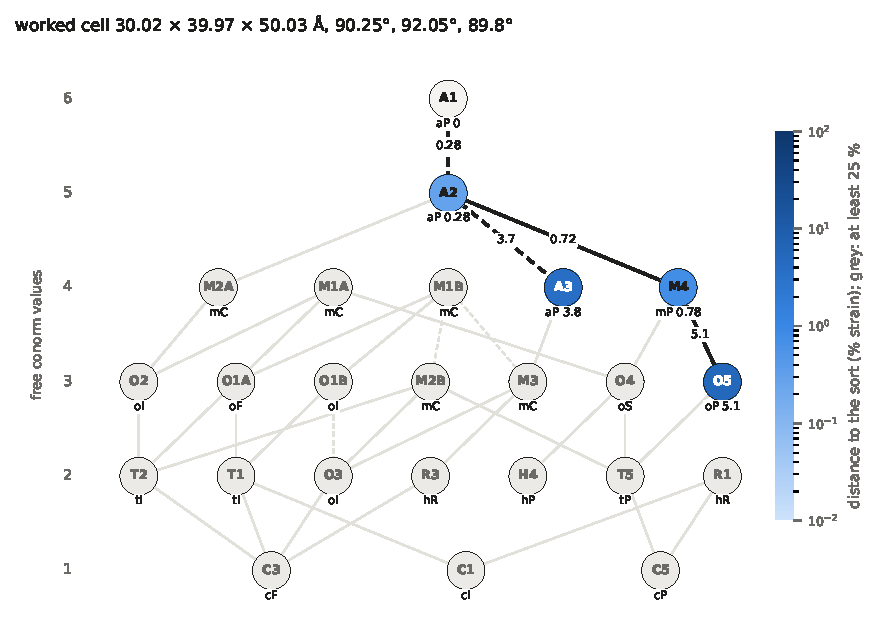
\includegraphics[width=0.9\textwidth]{figures/figS1_sort_graph.pdf}
\caption{The 24 Delone sorts as a graph for the measured worked cell. Rows are the number of free conorm values. Each node gives the Bravais type and the strain distance (\%) from the cell to the sort, its colour the same distance on a log scale; sorts at least $25\%$ away are grey. Edges are the specialisations of Table~\ref{tab:special}, labelled with the distance from the cell idealised onto the upper sort to the lower one. Dark edges are routes on which these steps add in quadrature to the lower sort's distance within $3\%$, drawn where that distance is below $10\%$. Dashed edges keep the Bravais type.}
\label{fig:sortgraph}
\end{figure}

\begin{figure}
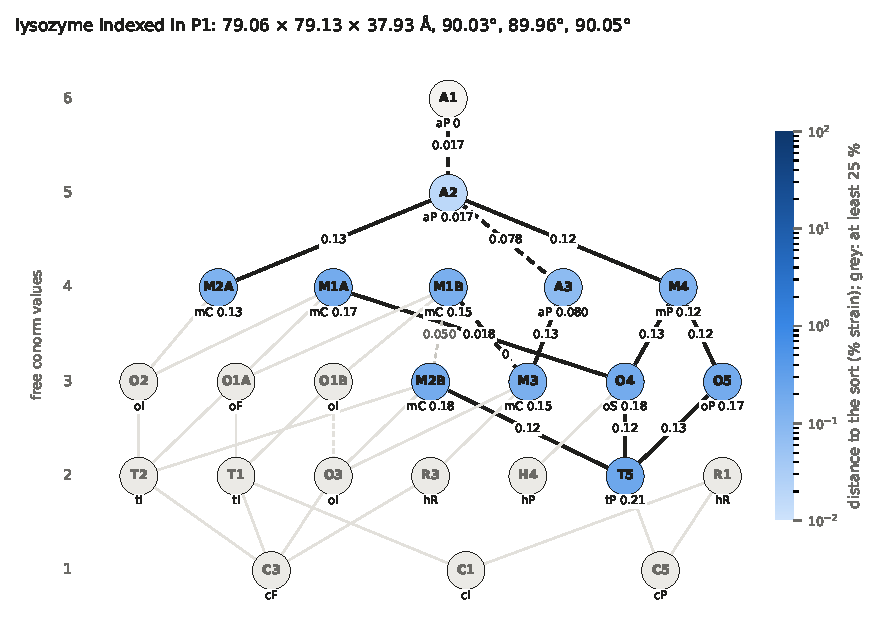
\includegraphics[width=0.9\textwidth]{figures/figS2_sort_graph_lysozyme.pdf}
\caption{The 24 Delone sorts as a graph for a tetragonal lysozyme cell ($79.1\times79.1\times37.9$\,\Ang) indexed in $P1$ with an added error, drawn as Fig.~\ref{fig:sortgraph}. The twelve sorts from aP to tP lie within $0.22\%$; every other sort is at least $25\%$ away (grey).}
\label{fig:lyso}
\end{figure}

\emph{Le Page's $3^\circ$ by sort.} The distance to a sort at Le Page's boundary depends on the sort, while the price of each operator does not. For exact lattices of each sort perturbed in random directions until Le Page's obliquity for the sort's Bravais group is exactly $3^\circ$, the median largest twofold price is $14.8\%$ in every sort, which Proposition~A9 makes true by construction and the table confirms numerically (larger only in the monoclinic tails, up to $40$--$55\%$, where Le Page's group is another C-centred group), while the median distance to the sort is $7.4$--$7.7\%$ for the orthorhombic and monoclinic sorts other than O3, M2B and M3, $7.9$--$8.1\%$ for tP, tI, hP and hR, and $8.3$--$8.5\%$ for the cubic sorts, with longer tails for the boundary sorts O3, M2B and M3 (Table~\ref{tab:lepage}). A single band on the distance to a sort therefore tests each sort at a different level, which is why the reindexing in this paper is decided on the prices of operators.

\begin{table}
\caption{Le Page's $3^\circ$ by Delone sort: for exact lattices of each sort, each perturbed in a random direction until the obliquity of the sort's Bravais group is $3^\circ$, the strain distance to the sort (median, and 10th--90th percentiles) and the median of the largest price of the lattice's twofolds and of its other rotations, by order, in \%. In the monoclinic sorts some perturbations reach the boundary through a different C-centred group, whose own twofold costs $14.8\%$ while the exact lattice's costs more. Of 25 directions per sort, those that never reach an obliquity of $3^\circ$ are dropped, hence $n<25$ in seven sorts; with $n\le25$ the percentiles are indicative.}
\label{tab:lepage}
\begin{footnotesize}
\begin{tabular}{llrlrl}
\toprule
sort & type & $n$ & distance to sort & twofold price & other orders \\
\midrule
C1 & cI & 25 & 8.3 (7.6--9.0) & 14.8 & 3: 14.1, 4: 15.0 \\
C3 & cF & 25 & 8.3 (7.7--9.2) & 14.8 & 3: 14.3, 4: 14.5 \\
C5 & cP & 25 & 8.5 (7.6--9.3) & 14.8 & 3: 14.2, 4: 14.7 \\
H4 & hP & 25 & 7.9 (7.5--8.5) & 14.8 & 3: 13.7, 6: 11.3 \\
T1 & tI & 25 & 7.9 (7.5--9.1) & 14.8 & 4: 14.0 \\
T2 & tI & 25 & 8.0 (7.6--8.8) & 14.8 & 4: 14.4 \\
T5 & tP & 25 & 8.0 (7.4--8.9) & 14.8 & 4: 14.1 \\
R1 & hR & 25 & 8.0 (7.5--8.6) & 14.8 & 3: 14.4 \\
R3 & hR & 25 & 8.1 (7.5--8.8) & 14.8 & 3: 14.5 \\
O1A & oF & 24 & 7.5 (7.4--7.8) & 14.8 & --- \\
O1B & oI & 25 & 7.6 (7.4--8.1) & 14.8 & --- \\
O2 & oI & 25 & 7.6 (7.4--8.2) & 14.8 & --- \\
O3 & oI & 25 & 8.6 (7.6--13.6) & 14.8 & --- \\
O4 & oS & 25 & 7.7 (7.4--8.2) & 14.8 & --- \\
O5 & oP & 25 & 7.5 (7.4--8.3) & 14.8 & --- \\
M1A & mC & 20 & 7.4 (7.4--9.1) & 14.8 & --- \\
M1B & mC & 15 & 7.4 (7.4--7.4) & 14.8 & --- \\
M2A & mC & 18 & 7.4 (7.4--8.5) & 14.8 & --- \\
M2B & mC & 17 & 9.3 (7.5--19.9) & 14.8 & --- \\
M3 & mC & 23 & 8.9 (7.5--16.1) & 14.8 & --- \\
M4 & mP & 23 & 7.4 (7.4--7.4) & 14.8 & --- \\
\bottomrule
\end{tabular}
\end{footnotesize}
\end{table}

\emph{Against BLDConograph and SELLA.} On the seven sample cells that Oishi-Tomiyasu (2024) distributes with BLDConograph, the highest Bravais type within $7.4\%$ is the program's type in all seven, with the next type at least $14.9\%$ away (Table~\ref{tab:conograph}). SELLA (\texttt{CmdSella}, Andrews \emph{et al.}, 2023, default settings) was run on the worked cell, the lysozyme cell, a pseudo-tetragonal cell, a cell with all angles $92^\circ$, a needle, two plates and the seven BLDConograph cells. The two rankings of the 24 sorts agree closely, with Spearman's rank correlation $0.77$ to $0.97$ over all 24 sorts, which the many distant sorts inflate. The two scales are not proportional: SELLA's distance divided by the cell's mean squared edge is a median $0.71$ times the strain distance, with a 10th to 90th percentile range of $0.05$ to $26$ (\texttt{results\_sella.txt}). With SELLA's band set by that median ratio, which is calibrated on the same 14 cells and so flatters the agreement, the Bravais types within the band agree in 11 of the 14 cells. They differ on the needle and the two plates, where the normalisation by the mean squared edge, our choice and not SELLA's, weighs the long edges differently: SELLA admits hP, hR, oF, tI and tP for the needle, which are far in strain, and the strain band admits oF (and tI) for the plates, which SELLA's does not. For these thin cells $r_1$ is $4$ to $6\%$, so their strain distances above it are bounds and are flagged.


%==============================================================================
\section{Computational checks}

{\sloppy Every check is a function of the package \texttt{sellingproofs} in the directory \texttt{manuscript/\allowbreak supplement} of the \texttt{agentsg} repository. A decorator, \texttt{@claim}, registers each function with the number z$nn$ of the statement it verifies, the places in the paper where the statement is made, and its kind: a machine-checked proof (formal), an exhaustive finite computation (exhaustive), spot checks on seeded samples (sampled), an exact rational certificate (certified), a number recomputed from the deposited results (benchmark, pdb), or a rerun of a script that regenerates its deposited results file (reproduce). The first paragraph of each function's documentation states the claim as the paper makes it. \texttt{python -m sellingproofs ledger} lists the claims and \texttt{python -m sellingproofs run} runs them as pytest tests; Table~\ref{tab:checks} is generated from the ledger. The statement groups are: % generated by python -m sellingproofs tables; do not edit
z36: from a metric error to a band on the conorms: coverage constants (2); z44: the band theorem: class excess, generation by flips, brute force (4); z45: the worked cell's widened set, walks and reduction under a band (1); z46: the closure groupoid of every sort, the monoclinic ring (8); z47: reindexing under a declared metric error (1); z48: Delone's sorts from the groupoid (1); z49: bands per slot, cell shapes as classical ambiguities (1); z50: codimension-one specialisations (2); z52: the operator set U: 6096 operators, kinds, entries (1); z53: sorts as closed subspaces (1); z54: the table of sorts from the operators (1); z55: exactness beyond the proved band (1); z56: the window lemma on all 38 faces, completeness of U (3); z57: bands per slot on needles and plates (2); z58: projection, enumeration and filtering, needles and plates (4); z59: balls, layers and adjacency radii (2); z60: strains, prices, symmetries and the worked cell (16); z61: the appendix statements: Voronoi characterisation, generation, A4, A10, A11 (8); z62: the machine-checked proofs (Lean) (31); z63: the implementation (library tests) (18); z64: the benchmark numbers and their reproduction (43); z65: the PDB numbers and their reproduction (25); z66: remaining statements, tables and figures (26); z67: the reindexing workflow: identities, worked example, comparison with the direct form (6); z68: the Niggli window and the way from a reduced cell to the Niggli cell (8).
 \texttt{python -m sellingproofs pin} prints the commit, the \texttt{agentsg} version (0.5.0) and the SHA-256 hashes of the two copies of $\mathcal U$, which a claim checks. The checks were run with Python 3.13.16, NumPy 2.5.3, SciPy 1.18.1 and cctbx-base 2025.11. A claim whose data or programs are absent is skipped with the reason, or fails when asked to (\texttt{--strict-needs}): the PDB claims need the Zenodo snapshot (doi:\allowbreak 10.5281/\allowbreak zenodo.22986222) in \texttt{data/}, the comparisons need cctbx and SELLA (CmdSella), and the formal claims Lean.\par}

\emph{Formal proofs.} The Lean development in \texttt{manuscript/\allowbreak supplement/\allowbreak formal} builds with Lean 4.35.0 and Mathlib release v4.35.0 (\texttt{lake build}). Its data file is generated from \texttt{universal\_\allowbreak operators\_\allowbreak columns.json} and records the file's SHA-256 hash, which \texttt{check\_data.py} recomputes. \texttt{audit/\allowbreak axioms.lean} prints the axioms of each headline theorem. Table~\ref{tab:lean} lists the theorems with the statements they prove. Beyond the three standard axioms of Lean's logic (\texttt{propext}, \texttt{Classical.\allowbreak choice}, \texttt{Quot.\allowbreak sound}), the completeness of $\mathcal U$ (\texttt{arrow\_\allowbreak mem\_U}, and \texttt{arrow\_\allowbreak mem\_U\_\allowbreak of\_\allowbreak posdef} for every lattice) depends on one compiled evaluation (\texttt{native\_decide}, of \texttt{finite\_\allowbreak check}); its converse (\texttt{U\_arrow}) on two (\texttt{U\_\allowbreak realised}, \texttt{U\_\allowbreak unimodular}); the dependence on the zero pattern (\texttt{arrow\_\allowbreak zero\_\allowbreak pattern} and \texttt{arrow\_\allowbreak zero\_\allowbreak pattern\_\allowbreak of\_\allowbreak posdef}) on two (\texttt{finite\_\allowbreak check}, \texttt{zero\_\allowbreak pattern\_\allowbreak check}); the size of $\mathcal U$, its distinct elements, its entries, the 38 zero patterns, and the closure of $\mathcal U$ under inversion and under the 48 relabellings on one each. That the non-zero conorms of a lattice connect the four vectors (\texttt{conn\_\allowbreak of\_\allowbreak posdef}), the window (\texttt{box\_\allowbreak of\_\allowbreak conn}, Lemma~A2 of the main text), Lemma~A1 (\texttt{excess\_\allowbreak identity}), the shortest partial sums (\texttt{partial\_\allowbreak shortest}), every part of Propositions~A10 and A9(i) (\texttt{price\_mul}, \texttt{price\_inv}, \texttt{coset\_\allowbreak lower}, \texttt{coset\_\allowbreak upper}, \texttt{Hgroup}, \texttt{candidates\_\allowbreak eq\_\allowbreak coset}, \texttt{stab\_\allowbreak sub\_H}, \texttt{H\_sub\_H}, \texttt{H\_\allowbreak eq\_\allowbreak stab}, \texttt{price\_\allowbreak le\_\allowbreak two\_\allowbreak dist\_\allowbreak fixed}, \texttt{twofold\_\allowbreak midpoint\_\allowbreak fixed}) and Proposition~A11(i)--(ii) depend on the standard axioms alone, that is, on the kernel.

\emph{What the formal statements assume.} The formal statements are narrower than, or equal to, the prose in the following ways, each of which the prose states or the text bridges. (i) Lattice vectors are coordinates in the basis $(a,b,c)$ of a reduced superbase with conorms $p\ge0$, and dot products are given by Selling's identity, so every statement about $\mathcal U$ is in the basis of the first superbase, which is how $\mathcal U$ is defined; since any obtuse superbase can serve as the first, this covers the matrices between any two. (ii) A lattice is a metric positive definite on the non-zero integer vectors; \texttt{conn\_\allowbreak of\_\allowbreak posdef} derives from it the connected support that \texttt{arrow\_\allowbreak mem\_U} assumes. (iii) The window is $[-7,7]^3$, wider than the $[-6,7]$ of the prose. (iv) Of the characterisation of obtuse superbases by shortest partial sums, the forward direction is proved for every metric (\texttt{partial\_\allowbreak shortest}); the converse, that a superbase whose partial sums are all shortest on a pattern is obtuse there, is checked for the elements of $\mathcal U$ by \texttt{zero\_\allowbreak pattern\_\allowbreak check}, which is all the completeness proof needs. (v) Propositions~A9(i) and A10 are proved for any isometric action of a group on a metric space, with the price the displacement $\dist(x,g\cdot x)$; they apply to the paper's prices because a unimodular change of basis is an isometry of the affine-invariant distance between metrics normalised to unit determinant (Section~3.4 of the main text), which is not formalised. The order of products follows the left action $g\cdot\Gmet=g^{-\mathsf T}\Gmet g^{-1}$, under which the paper's $h\Pop_0$ is written $\Pop_0h$. (vi) The equality case of Proposition~A9(i) assumes that the midpoint of $\Gmet$ and $g^{\mathsf T}\Gmet g$ exists and is unique, which holds in the space of positive definite matrices (Bhatia, 2007) but is not formalised. (vii) Proposition~A11 is formalised in the Gram entries of the cell, with Niggli's main conditions only, which is how it is stated.

\begin{table}
\caption{The machine-checked theorems (Lean~4 with Mathlib, in \texttt{manuscript/\allowbreak supplement/\allowbreak formal}): the statement each proves, where the paper makes it, and the compiled evaluations (\texttt{native\_decide}) it rests on beyond the three standard axioms. Generated from the package's ledger (claim z62), which builds the development and checks each theorem's axioms.}
\label{tab:lean}
\begin{scriptsize}
\begin{tabular}{>{\raggedright\arraybackslash}p{3.2cm}>{\raggedright\arraybackslash}p{2.2cm}>{\raggedright\arraybackslash}p{6.4cm}>{\raggedright\arraybackslash}p{2.8cm}}
\toprule
theorem & place & statement & compiled evaluations \\
\midrule
\csname @@input\endcsname checks_lean.tex 
\bottomrule
\end{tabular}
\end{scriptsize}
\end{table}

\emph{Certified radii.} The depth of a superbase $F$ with conorms $q$ under the metric is the least strain norm $\|r\|_M$ of a change $r\ge-q$ of its conorms, with $M$ the strain norm in the basis of $F$ ($r^{\mathsf T}Mr=\mathrm{tr}(\Gmet^{-1}\Delta\Gmet\,\Gmet^{-1}\Delta\Gmet)$). For any multipliers $\lambda\ge0$ with $c=-\lambda\cdot q>0$ the depth is at least $c/(\lambda^{\mathsf T}M^{-1}\lambda)^{1/2}$, by weak duality, and any $r$ with $q+r\ge0$ whose metric is positive definite bounds it from above. \texttt{certify\_radii.py} evaluates the balls of Lemma~A6 and the conorm test of Proposition~A4 exactly, so that every superbase within the cap is among its candidates, proves a lower bound for every candidate outside the layer and an upper bound for the nearest, all in rational arithmetic; floating point only proposes $\lambda$ and $r$. The certificates are for the reduced conorms as stored in double precision, read as exact rationals, which agree with the cells of Table~8 to about 15 digits.

\emph{Timings.} On a tenth of the benchmark, widening a reference took a median of $0.02$\,s and reindexing one new cell $0.03$\,s ($90$th percentiles $0.03$ and $0.12$\,s); a $150\times120\times4.8$\,\Ang\ plate took $0.9$\,s to widen. A $300\times300\times3$\,\Ang\ plate takes about a minute to widen and its $r_1$ several minutes, and thinner cells are refused by the cap on the ball. A vectorised lookup of $\mathcal U$ for one new cell, reductions included, takes about $0.04$\,s (\texttt{adjacency\_radii.py}).

\begin{table}
\caption{The checks behind each place in the paper: the numbers z$nn$ of the statement groups whose checks cite it, and the number of checks. Generated by \texttt{python -m sellingproofs tables} from the ledger of the package; the subjects of the groups are listed in the text.}
\label{tab:checks}
\begin{scriptsize}
\begin{tabular}[t]{>{\raggedright\arraybackslash}p{2.3cm}>{\raggedright\arraybackslash}p{3.6cm}r}
\toprule
main text & statements & checks \\
\midrule
\csname @@input\endcsname checks_main.tex 
\bottomrule
\end{tabular}\hfill
\begin{tabular}[t]{>{\raggedright\arraybackslash}p{2.3cm}>{\raggedright\arraybackslash}p{3.6cm}r}
\toprule
supporting information & statements & checks \\
\midrule
\csname @@input\endcsname checks_si.tex 
\bottomrule
\end{tabular}
\end{scriptsize}
\end{table}



%==============================================================================
\section{Existing searches on the same cases}\label{si:searches}

The test cases of the main text were also given to the searches that data-processing programs use, each priced in the same way and kept within the same band: every matrix with entries in $\{-1,0,1\}$ or $\{-2,\dots,2\}$ between the two Selling-reduced cells; the $\{-1,0,1\}$ search between the two Niggli cells; cctbx \texttt{similarity\_\allowbreak transformations} between the two Niggli cells (Grosse-Kunstleve \emph{et al.}, 2002) with generator ranges 1 and 2; and a pipeline that runs the cctbx lattice-symmetry analysis (Sauter \emph{et al.}, 2004) on both cells and returns every operation of the reference's highest lattice group between the two standard settings. Table~\ref{tab:searches} gives the counts. The searches between Niggli cells and the cctbx similarity searches found the true operator in every case; the fixed windows between Selling-reduced cells, which no program uses, miss operators where Table~4 of the main text says they can; the pipeline missed a needle whose reference and measured cell idealise at $3^\circ$ to different lattices, and a few stress and window cases. The purpose of the table is to show that the guarantee and the existing searches agree where both apply, not to rank them.

\begin{table}
\caption{Existing searches on the test cases of the main text (Section~4.4): the true operator among the candidates, by method and family; candidates priced by the geodesic distance after the best scale and kept within a band of $7.4\%$ (the reference widened at $7.7\%$ for the closure and the lookup). Window family: cells measured in a member that needs an entry of $3$, and near-mP and near-orthogonal lattices measured twice with an error of $0.1$ to $2\%$, the reference given as its Niggli cell (split by Niggli type) or in a random basis (split by the kind of face). A dash: not run. The lookup on the benchmark and stress families is in \texttt{results\_lookup.txt}. Results in \texttt{manuscript/\allowbreak supplement/\allowbreak benchmark/}.}
\label{tab:searches}
\begin{footnotesize}
\setlength{\tabcolsep}{3pt}\begin{tabular}{lrrrrrrrr}
\toprule
 & & & & & \multicolumn{4}{c}{2- or 3-zero faces, reference given as} \\
 & & \multicolumn{2}{c}{stress} & & \multicolumn{2}{c}{Niggli cell} & \multicolumn{2}{c}{random basis} \\
method & benchmark & $0.5\epsilon$ & $0.9\epsilon$ & entry $3$ & type~I & type~II & 2 zeros & 3 zeros \\
\midrule
closure & 780/780 & 60/60 & 60/60 & 60/60 & 171/171 & 129/129 & 150/150 & 150/150 \\
lookup of $\mathcal U$ & 780/780 & 60/60 & 60/60 & 60/60 & 171/171 & 129/129 & 150/150 & 150/150 \\
$\{-1,0,1\}$, Selling cells & 778/780 & 58/60 & 52/60 & 24/60 & 142/171 & 129/129 & 120/150 & 99/150 \\
$\{-2,\dots,2\}$, Selling cells & 780/780 & 59/60 & 60/60 & 52/60 & 170/171 & 129/129 & 150/150 & 149/150 \\
$\{-1,0,1\}$, Niggli cells & 780/780 & 60/60 & 60/60 & 60/60 & 171/171 & 129/129 & 150/150 & 150/150 \\
cctbx similarity, range 1 & 780/780 & 60/60 & 60/60 & 60/60 & 171/171 & 129/129 & 150/150 & 150/150 \\
cctbx similarity, range 2 & 780/780 & 60/60 & 60/60 & 60/60 & 171/171 & 129/129 & 150/150 & 150/150 \\
lattice-symmetry pipeline & 779/780 & 56/60 & 54/60 & 60/60 & 171/171 & 126/129 & 147/150 & 148/150 \\
\bottomrule
\end{tabular}
\end{footnotesize}
\end{table}


%==============================================================================
\section{Uncertainty of the PDB statistics, chance, and the Niggli window}\label{si:pdbstats}

\emph{Intervals.} Table~\ref{tab:bootstrap} gives block-bootstrap 95\% intervals for the percentiles of Table~10 of the main text: the deposition blocks (runs of id-adjacent pairs) are resampled with replacement, 1000 times, which keeps the correlation within a deposition series. The shares of entries with an alternative within the band have intervals of $\pm0.2$ to $\pm0.5$ points, where a type with fewer than 200 blocks uses the pooled band (\texttt{pdb\_band\_uncertainty.py}).

\begin{table}
\caption{Non-isomorphism in the PDB by reported Bravais type with block-bootstrap 95\% intervals (cut $20\%$, identity as the operator, price after the scale fit, \%). $^a$Fewer than 200 deposition blocks; the pooled band stands in for these types in the shares of the main text, and the cubic rows are zero by construction.}
\label{tab:bootstrap}
\begin{footnotesize}
\begin{tabular}{lrrlll}
\toprule
type & pairs & blocks & median & 90th & 95th \\
\midrule
aP & 902 & 535 & 2.06 (1.82--2.27) & 7.66 (6.40--9.46) & 11.68 (9.76--13.70) \\
mP & 7\,077 & 3\,277 & 1.27 (1.21--1.33) & 5.38 (5.01--5.84) & 9.02 (8.21--9.78) \\
mC & 4\,932 & 1\,977 & 1.49 (1.41--1.59) & 5.06 (4.73--5.49) & 8.40 (7.16--9.23) \\
oP & 13\,615 & 5\,987 & 1.11 (1.07--1.14) & 4.70 (4.46--4.95) & 7.43 (7.06--7.81) \\
oS & 2\,271 & 1\,108 & 1.01 (0.94--1.08) & 3.57 (3.32--4.01) & 5.50 (4.96--6.14) \\
oI & 1\,353 & 574 & 1.22 (1.07--1.39) & 5.12 (4.28--6.16) & 7.91 (6.40--9.15) \\
oF$^a$ & 31 & 22 & 1.99 (1.23--3.10) & 5.87 (3.39--8.28) & 7.54 (4.48--8.95) \\
tP & 5\,174 & 2\,061 & 0.52 (0.48--0.57) & 2.59 (2.36--2.85) & 4.00 (3.61--4.41) \\
tI & 805 & 416 & 0.65 (0.53--0.78) & 2.76 (2.28--3.34) & 4.91 (3.61--6.03) \\
hR & 1\,270 & 597 & 0.68 (0.61--0.79) & 3.54 (3.10--3.94) & 5.86 (4.59--6.71) \\
hP & 6\,817 & 3\,167 & 0.57 (0.53--0.62) & 2.87 (2.65--3.04) & 4.56 (4.22--4.95) \\
cP$^a$ & 363 & 178 & 0.00 (0.00--0.00) & 0.00 (0.00--0.00) & 0.00 (0.00--0.00) \\
cI$^a$ & 385 & 194 & 0.00 (0.00--0.00) & 0.00 (0.00--0.00) & 0.00 (0.00--0.00) \\
cF$^a$ & 211 & 106 & 0.00 (0.00--0.00) & 0.00 (0.00--0.00) & 0.00 (0.00--0.00) \\
all & 45\,222 & 20\,206 & 0.98 (0.96--1.00) & 4.21 (4.09--4.33) & 6.72 (6.52--6.98) \\
\bottomrule
\end{tabular}
\end{footnotesize}
\end{table}

\emph{Against chance.} Shuffling the free cell parameters independently among the entries of one space group keeps their distributions and destroys any relation between them; shuffling within twenty classes of cell volume keeps cells of one size together. At Le Page's $3^\circ$ the real rate exceeds both shuffled ones for $P1$ ($42$--$44\%$ against $30$--$40\%$) and $P2_12_12_1$ ($23$--$24\%$ against $13$--$17\%$), whose real cells are more often pseudo-tetragonal, exceeds them slightly for $P2_1$ ($46\%$ against $39$--$44\%$), and matches them for $C2$ and $P2_12_12$. Near-exact pseudo-symmetry is not chance: the share whose cheapest alternative costs at most $1\%$ is $10\%$ for real $P1$ cells against $2$--$3\%$ shuffled, and $9\%$ against $5$--$6\%$ for $P2_1$ (intervals about $\pm1$ point). At $4.2\%$ the excess remains for $P1$ ($15$--$16\%$ against $6$--$9\%$) but not clearly for $P2_1$ ($18\%$ against $13$--$18\%$, intervals about $\pm2$ points), and mP entries carry much of the share within $4.2\%$ (two draws of 1500 cells per arm; \texttt{results\_\allowbreak pdb\_\allowbreak lepage\_\allowbreak null.txt}).

\emph{The crystal-form proxy.} Random pairs of entries with one space group whose identifiers do not share their first three characters, drawn with the space-group mix of the id-adjacent pairs, pass the $20\%$ cut in $1.5\%$ of 19\,986 cases ($0.75\%$ at $5\%$; \texttt{pdb\_\allowbreak proxy\_\allowbreak check.py}). Unrelated crystals rarely pass the cut by chance, so the movement of the percentiles with the cut reflects variation within deposition series rather than unrelated pairs.

\emph{The Niggli window.} \texttt{niggli\_window.py} draws 100 lattices on each of the 38 faces (half of them anisotropic, with vertex scales up to 30) and on each of the 24 sorts, measures each twice with independent errors of total strain $0.5$, $2$, $5$ and $7.7\%$, the new cell in a random basis, and computes the true operator between the two Niggli cells (cctbx) and between the two Selling-reduced cells directly. Between Niggli cells its entries were in $\{-1,0,1\}$ in all 24\,800 cases, strictly and not only up to the lattice's point group, and in 3\,040 further cases on strongly anisotropic lattices (\texttt{niggli\_window.py thin}: 40 per face, vertex scales up to 60, the square root of the metric's eigenvalue ratio up to 98, median 5); between Selling-reduced cells an entry of 2 or 3 was needed in 3\,765 cases (on two zeros sharing a vector, three zeros, and the sorts cP, tP and oP) and in none once composed with the point group. Proposition~A12 of the main text turns the first observation into a theorem for exact lattices and for measurements within a radius $\rho$ of one lattice (Section~\ref{si:niggli}).

%==============================================================================
\section{The reindexing workflow in detail}\label{si:workflow}

This section sets out, step by step, how the candidates of Section~4.2 of the main text are computed for a new cell once a reference has been widened, why each step is exact, what it costs, and what it gives on the worked cell. The procedure prices exactly the operators that the direct form of Table~7 of the main text prices, the operator $\Pop=B_R\Wop_k\mathbf QB_N^{-1}$ for every member $\Wop_k$ of the reference's widened set and every relabelling $\mathbf Q$; it differs only in where the work is done. Four observations reorganise it. (i) The two input bases drop out of every price, so each candidate can be priced in the new cell's reduced basis from a metric that depends only on the reference. (ii) Of the 48 relabellings of a superbase, two that differ by a common sign give the same metric, and the determinant rule keeps exactly one of them, so there are 24 metrics per member. (iii) Every candidate has the same best scale. (iv) A necessary condition on ten dot products of the new cell's reduced superbase, which follows from Lemma~A7(i) and Proposition~A4 of the main text, discards almost every ordering before an eigenvalue is computed. The exact operator is then built only for the candidates that lie within the band. The workflow is implemented in \texttt{agentsg} as the reindexing routine; a second entry point, \texttt{reindex\_workflow}, returns every intermediate quantity named below, and the numbers of this section are produced by \texttt{reindex\_workflow.py} (\texttt{results\_\allowbreak reindex\_\allowbreak workflow.txt}) and checked by claim z67 and by the library test registered as z63 (Section~S7).

\subsection{Notation}

The reference $R$ is given as a cell and a space group. Its primitive cell is Selling-reduced (step~1 of Table~7 of the main text), which gives the reduced basis $B_R$, a $3\times3$ matrix whose columns are the reduced basis vectors $a,b,c$ written in the reference's input basis, and the reduced metric
\begin{equation}
\Gmet_R=B_R^{\mathsf T}\,\Gmet_R^{\rm in}\,B_R ,
\end{equation}
with $\Gmet_R^{\rm in}$ the metric of the input cell. $B_R$ is integer for a primitive input cell and rational, with determinant $\pm1/k$, for a centred cell in its conventional basis. The reduced superbase is $F_0=(d,a,b,c)$, $d=-a-b-c$; in the reduced basis its four vectors are the rows $(-1,-1,-1)$, $(1,0,0)$, $(0,1,0)$, $(0,0,1)$. The reference's widened set at strain $\eta=e^\epsilon-1$ for the price band $\epsilon$ has members $F_1,\dots,F_m$; each is a superbase of four integer vectors, written as rows in the reference's reduced basis, with a depth, the strain from $\Gmet_R$ to the nearest metric that makes it obtuse. The new cell $N$ is reduced in the same way, which gives $B_N$, $\Gmet_N^{\rm in}$ and $\Gmet_N=B_N^{\mathsf T}\Gmet_N^{\rm in}B_N$. The price of an operator $\Pop$ is
\begin{equation}
\pi(\Pop)=\min_{s>0}\,\dist\!\bigl(\Gmet_N^{\rm in},\,s\,\Pop^{\mathsf T}\Gmet_R^{\rm in}\Pop\bigr),
\label{eq:wf-price}
\end{equation}
with $\dist$ the geodesic distance of equation~(3) of the main text.

\subsection{Step 1: the member table}

\emph{Ordered bases.} A superbase $F=(v_0,v_1,v_2,v_3)$ has 48 labelled bases: leave out one of the four vectors, put the other three in an order, and give them a common sign $c=\pm1$. Write $B$ for the $3\times3$ integer matrix whose rows are the three vectors in order, without the sign; there are $4\times3!=24$ such \emph{ordered bases} per superbase, and the 48 labelled bases are $cB$. Every $B$ is unimodular, since three vectors of a superbase form a basis of the lattice.

\emph{Their metrics.} The column operator of the labelled basis $cB$ is $\Wop=cB^{\mathsf T}$, and the metric it predicts for the new cell's reduced basis is
\begin{equation}
\mathbf H=\Wop^{\mathsf T}\Gmet_R\Wop=c^2\,B\,\Gmet_R\,B^{\mathsf T}=B\,\Gmet_R\,B^{\mathsf T},
\label{eq:wf-H}
\end{equation}
which does not depend on the sign. A member therefore predicts 24 metrics, not 48. The member table holds, for every member $k$ and ordered basis $o$, the matrix $B_{ko}$, its determinant $\det B_{ko}=\pm1$, and $\mathbf H_{ko}$; it is computed once per reference and serves every new cell compared with it. In the conorm language of Section~2 of the main text, $\mathbf H_{ko}$ is the metric whose reduced superbase has the six conorms of $F_k$ in the slot order that the ordering $o$ induces, so the table is the member's six conorms under the 24 permutations of the four vectors.

\subsection{Step 2: the new cell, and why the input bases drop out}

The new cell is reduced once. For $\Pop=B_R\Wop B_N^{-1}$,
\begin{equation}
\Pop^{\mathsf T}\Gmet_R^{\rm in}\Pop=B_N^{-\mathsf T}\,\Wop^{\mathsf T}\bigl(B_R^{\mathsf T}\Gmet_R^{\rm in}B_R\bigr)\Wop\,B_N^{-1}=B_N^{-\mathsf T}\,\mathbf H\,B_N^{-1},\qquad \Gmet_N^{\rm in}=B_N^{-\mathsf T}\,\Gmet_N\,B_N^{-1}.
\end{equation}
Both metrics in equation~(\ref{eq:wf-price}) are transformed by the same congruence $X\mapsto B_N^{-\mathsf T}XB_N^{-1}$, an isometry of $\dist$ (main text, Section~3.4); equivalently, $(\Gmet_N^{\rm in})^{-1}\Pop^{\mathsf T}\Gmet_R^{\rm in}\Pop=B_N\,\Gmet_N^{-1}\mathbf H\,B_N^{-1}$ is similar to $\Gmet_N^{-1}\mathbf H$ and has the same eigenvalues. Hence
\begin{equation}
\pi(\Pop)=\min_{s>0}\dist(\Gmet_N,\,s\,\mathbf H),
\label{eq:wf-reduced}
\end{equation}
the comparison of the new cell's reduced metric with an entry of the member table. Neither input basis, nor the rational part of a centred reference's $B_R$, enters a price. The implementation forms $\Gmet_R$ and $\Gmet_N$ from the input cells exactly as written, so that the prices agree with the direct form to rounding.

\subsection{Step 3: the determinant rule}

$\det\Pop=\det B_R\,c^3\det B\,/\det B_N$, so the sign of $\det\Pop$ is $c\,\det B\,\operatorname{sgn}(\det B_R)\operatorname{sgn}(\det B_N)$. For a proper operator (main text, Section~4.2) the sign $c$ is therefore fixed by the ordered basis,
\begin{equation}
c=\det B\;\operatorname{sgn}(\det B_R)\,\operatorname{sgn}(\det B_N),
\end{equation}
and every ordered basis gives exactly one proper candidate: $24m$ candidates for $m$ members, each with its own metric. For a reference whose widened set is the whole first layer, $m=127$ and $24\times127=3048$, the proper half of $\mathcal U$ that the lookup of Remark~A8 tries (Table~7 of the main text, step~3). When improper operators are asked for, the other sign is taken; when both are, both are listed, with the same price.

\subsection{Step 4: one scale for every candidate}

Every $\mathbf H_{ko}$ has $\det\mathbf H_{ko}=(\det B_{ko})^2\det\Gmet_R=\det\Gmet_R$. With $l_1,l_2,l_3$ the logarithms of the eigenvalues of $\Gmet_N^{-1/2}\mathbf H\,\Gmet_N^{-1/2}$, $\dist(\Gmet_N,s\mathbf H)^2=\sum_i(l_i+\ln s)^2$, which is smallest at $\ln s=-\bar l$, $\bar l=\frac13\sum_il_i=\frac13\ln(\det\mathbf H/\det\Gmet_N)$. So the best scale
\begin{equation}
s=\Bigl(\frac{\det\Gmet_N}{\det\Gmet_R}\Bigr)^{1/3}
\label{eq:wf-scale}
\end{equation}
is the same for every candidate, and the price is $\pi=\bigl(\sum_i(l_i-\bar l)^2\bigr)^{1/2}$. The limit on the fitted change of edge lengths, $|\sqrt s-1|\le10\%$, is therefore one test for the pair of cells, not one per candidate; since the ratio of the primitive volumes is $V_N/V_R=s^{3/2}$, it is the volume check of step~2 of Table~7 of the main text, $(0.9)^3<V_N/V_R<(1.1)^3$, up to the treatment of the boundary.

\subsection{Step 5: a necessary condition on ten dot products}

\emph{The condition.} Let $u_0,\dots,u_3$ be the four vectors of the new cell's reduced superbase, with dot products $u_i\cdot u_j$ under $\Gmet_N$, lengths $|u_i|$ under $\Gmet_N$, and dot products $u_i^{\mathsf T}\mathbf H u_j$ under a predicted metric. If $\pi\le\epsilon$, then
\begin{equation}
\bigl|\,s\,u_i^{\mathsf T}\mathbf Hu_j-u_i^{\mathsf T}\Gmet_Nu_j\,\bigr|\le\eta\,|u_i|\,|u_j|\qquad(0\le i\le j\le3),\qquad\eta=e^\epsilon-1 .
\label{eq:wf-condition}
\end{equation}
\emph{Proof.} By step~4, $\pi=\dist(\Gmet_N,s\mathbf H)$. By Lemma~A7(i) of the main text with $\mathbf A=\Gmet_N$ and $\mathbf B=s\mathbf H$, $\|s\mathbf H-\Gmet_N\|_{\Gmet_N}\le e^{\pi}-1\le\eta$. By Proposition~A4 of the main text with the metric $\Gmet_N$ and the perturbation $\Delta\Gmet=s\mathbf H-\Gmet_N$, $|u^{\mathsf T}\Delta\Gmet\,v|\le\eta|u||v|$ for all vectors $u,v$, in particular for $u_i,u_j$.\hfill$\square$

The condition is exact, not a first-order estimate, and it never discards an ordering within the band. It reads the new cell's six conorms $p_{ij}=-u_i\cdot u_j$ and four squared lengths against the member's conorms in the slot order of the ordering, scaled by $s$: each conorm may differ by at most $\eta|u_i||u_j|$ and each squared length by $\eta|u_i|^2$. All ten bounds are computed once per new cell, and the predicted dot products $u_i^{\mathsf T}\mathbf H_{ko}u_j$ are entries of the member table, so the test costs ten comparisons per ordering. To absorb rounding, the implementation widens each bound by a relative $10^{-12}$ and an absolute $10^{-9}\max|u_i\cdot u_j|$, which only lets more orderings through.

\emph{Why it is selective.} A wrong ordering puts a large conorm of the member in a slot where the new cell has a small one, or the reverse, and conorms of a reduced cell differ by much more than $\eta$ times the product of lengths unless the cell is close to a symmetry that exchanges them. In the cases examined here an ordering passes when it is the true one, when it differs from the true one by an exact or near symmetry of the lattice, or when the member lies at a depth below about the band; the last two are the alternatives that a band is meant to report.

\subsection{Step 6: the prices}

For the orderings that pass, the eigenvalues of $\Gmet_N^{-1/2}\mathbf H_{ko}\Gmet_N^{-1/2}$ are computed in one batch ($3\times3$ symmetric eigenvalue problems), and $\pi=\|l-\bar l\mathbf 1\|$. Orderings with $\pi>\epsilon$ are dropped; with the scale fit switched off, $\bar l$ is replaced by $0$ and $s$ by $1$ in steps~4 to~6.

\subsection{Step 7: the exact operators}

For each ordering within the band the exact operator is built in rational arithmetic,
\begin{equation}
\Pop=B_R\,\bigl(c\,B_{ko}^{\mathsf T}\bigr)\,B_N^{-1},
\end{equation}
with the sign of step~3; then $(a_N\,b_N\,c_N)=(a_R\,b_R\,c_R)\Pop$, $\Gmet_N^{\rm in}\approx s\Pop^{\mathsf T}\Gmet_R^{\rm in}\Pop$ and $h_N=\Pop^{\mathsf T}h_R$ (main text, equation~(5)). Each candidate carries its price, the scale $s$, the depth of its member and its determinant. Two different pairs $(k,o)$ cannot give the same $\Pop$: three ordered vectors determine the superbase they belong to, and the members are distinct superbases; the implementation checks for repeats all the same. The candidates are listed by price, ties nearest the identity first, as in the direct form, and are then grouped into indexing classes (step~5 of Table~7; main text, Section~5.3).

\subsection{Why the result is the direct form's}

The direct form prices $\pi(B_R\,cB^{\mathsf T}B_N^{-1})$ for every member, ordered basis and sign. By step~2 each such price is $\min_s\dist(\Gmet_N,s\mathbf H_{ko})$, by step~3 the sign only decides whether the operator is proper, by step~4 the minimising scale is the common $s$, and by step~5 an ordering discarded by the necessary condition has $\pi>\epsilon$. The workflow therefore returns exactly the operators of the direct form within the band, with the same prices up to rounding; the completeness of the candidate set (Lemma~A7 and the completeness of $\mathcal U$) carries over unchanged. On the 780 cases of the benchmark the two return the same set of operators in every case, and on 24 cases with centred references (four new cells in random primitive bases for each of $C121$, $I222$, $R3$ on hexagonal axes, $F23$, $I4_1$ and $Fddd$) as well. The prices agree to $3\times10^{-12}$; the workflow gives exactly equal prices to operators related by a symmetry of the reference, since they share a predicted metric, where the direct form's products of rational and floating-point matrices differ in the last digits.

\subsection{Cost}

\begin{table}
\caption{The work of one reindexing, for a reference with $m$ members, in the direct form and in the workflow, with the counts for the worked cell (Table~\ref{tab:wf-example}) and, in parentheses, the medians and the totals over the 780 cases of the benchmark.}
\label{tab:wf-cost}
\begin{footnotesize}
\begin{tabular}{>{\raggedright\arraybackslash}p{4.4cm}>{\raggedright\arraybackslash}p{3.8cm}>{\raggedright\arraybackslash}p{5.6cm}}
\toprule
 & direct form & workflow \\
\midrule
once per reference & -- & member table: $24m$ ordered bases and metrics (384) \\
exact operators built & $48m$ (768; 238\,224 in all) & those within the band (2; 5\,797 in all) \\
dot-product conditions & -- & $10\times24m$ comparisons (3\,840; median 72 orderings) \\
eigenvalue problems & $48m$ (768) & orderings that pass (4; median 4, $5.9\%$ of all) \\
time for the 780 new cells & about 27\,s & about 1.3\,s \\
\bottomrule
\end{tabular}
\end{footnotesize}
\end{table}

The direct form builds and prices an exact rational operator for each of the $48m$ labelled bases. The workflow builds the member table once per reference, $24m$ integer matrices and $3\times3$ products; for each new cell it computes two determinants, ten bounds and $24m$ sets of ten comparisons, solves an eigenvalue problem only for the orderings that pass, and builds exact operators only within the band (Table~\ref{tab:wf-cost}). On the benchmark the members number 3 at the median and 56 at most, the orderings 72 at the median and 1\,344 at most; $5.9\%$ of the orderings pass the condition (median 4 per case, at most 64), and the work of building exact operators falls from 238\,224 to 5\,797, which is also the number of operators returned. The 780 reindexings took about 27\,s in the direct form and about 1.3\,s in the workflow on the same machine, a factor of about 20; the reference was widened beforehand in both, and the times depend on the machine.

\subsection{The worked cell}

\begin{table}
\caption{The workflow on the worked cell: the reference $30.02\times39.97\times50.03$\,\Ang, $90.25$, $92.05$, $89.80^\circ$ at the default price band, and as new cell the same lattice in the basis $(a,\,b,\,a+c)$ with an added strain of $0.3\%$. Conorms in \Ang$^2$ in the slot order $da,db,dc,ab,ac,bc$.}
\label{tab:wf-example}
\begin{footnotesize}
\begin{tabular}{>{\raggedright\arraybackslash}p{4.6cm}>{\raggedright\arraybackslash}p{9.6cm}}
\toprule
quantity & value \\
\midrule
price band $\epsilon$; strain $\eta=e^\epsilon-1$ & $0.0740$; $0.076807$ \\
reference: $B_R$, $\det B_R$ & $((-1,0,1),(0,1,0),(0,0,1))$, $-1$ \\
reference conorms & $49.54$, $1588.88$, $2444.74$, $4.19$, $847.47$, $4.54$ \\
widened set; layer & 16 members (Table~\ref{tab:wf-members}); first layer \\
new cell & $30.0319$, $40.0110$, $57.4349$\,\Ang; $90.0718$, $60.5600$, $89.8328^\circ$ \\
new cell: $B_N$, $\det B_N$ & $((1,0,0),(0,0,-1),(0,-1,0))$, $-1$ \\
new conorms & $50.61$, $2448.09$, $1594.50$, $847.80$, $3.51$, $2.88$ \\
step 1: ordered bases & $16\times24=384$, each with one proper sign (step 3) \\
step 4: common scale $s$; $\sqrt s$ & $1.001225$; $1.000612$, within $10\%$ \\
step 5: bounds $\eta|u_i||u_j|$, rows and columns $d,a,b,c$ & $(314.4, 147.6, 282.2, 196.6)$, $(147.6, 69.3, 132.5, 92.3)$, $(282.2, 132.5, 253.4, 176.5)$, $(196.6, 92.3, 176.5, 123.0)$ \\
step 5: orderings that pass & 4 of 384 (Table~\ref{tab:wf-priced}) \\
step 6: within the band & 2 \\
step 7: operators & $((1,0,1),(0,1,0),(0,0,1))$, price $0.212\%$, the true one; $((-1,0,-1),(0,1,0),(0,0,-1))$, price $1.381\%$, the pseudo-twofold \\
direct form & 768 exact operators built, the same two returned, prices equal to $7\times10^{-16}$ \\
\bottomrule
\end{tabular}
\end{footnotesize}
\end{table}

\begin{table}
\caption{The 16 members of the worked cell's widened set at the default band: their depths (strain to the nearest metric that makes them obtuse) and their conorms (\Ang$^2$) under the reference metric, in each member's stored labelling. The members are those of Table~\ref{tab:filter} in another order and labelling; the conorms agree up to a permutation of the slots. The first six form the ring of Fig.~1 of the main text; the others lie at depths of $3.8$ to $5.1\%$.}
\label{tab:wf-members}
\begin{footnotesize}
\begin{tabular}{rrrrrrrr}
\toprule
member & depth (\%) & \multicolumn{6}{c}{conorms} \\
\midrule
0 & 0.000 & $2444.7$ & $1588.9$ & $49.5$ & $4.5$ & $847.5$ & $4.2$ \\
1 & 0.280 & $852.0$ & $1593.4$ & $45.0$ & $-4.5$ & $2449.3$ & $8.7$ \\
2 & 0.494 & $8.7$ & $2440.6$ & $53.7$ & $1593.1$ & $-4.2$ & $851.7$ \\
3 & 0.617 & $2458.0$ & $-8.7$ & $53.7$ & $1602.1$ & $843.3$ & $4.2$ \\
4 & 0.777 & $847.5$ & $-4.2$ & $57.9$ & $-4.5$ & $2453.8$ & $1606.3$ \\
5 & 0.777 & $2449.3$ & $-8.7$ & $62.5$ & $4.5$ & $842.9$ & $1601.8$ \\
6 & 3.757 & $-49.5$ & $2494.3$ & $1638.4$ & $53.7$ & $897.0$ & $-45.0$ \\
7 & 4.561 & $-62.5$ & $2511.7$ & $53.7$ & $1664.2$ & $905.4$ & $-57.9$ \\
8 & 5.056 & $1584.7$ & $950.7$ & $2548.0$ & $4.2$ & $8.7$ & $-53.7$ \\
9 & 5.078 & $1539.3$ & $49.5$ & $2494.3$ & $905.4$ & $62.5$ & $-53.7$ \\
10 & 5.078 & $12.9$ & $954.9$ & $2543.8$ & $-4.2$ & $1588.9$ & $-49.5$ \\
11 & 5.091 & $12.9$ & $2556.7$ & $942.0$ & $-8.7$ & $1593.4$ & $-45.0$ \\
12 & 5.091 & $1548.4$ & $897.0$ & $45.0$ & $57.9$ & $2511.7$ & $-53.7$ \\
13 & 5.111 & $-12.9$ & $967.8$ & $2556.7$ & $1601.8$ & $8.7$ & $-62.5$ \\
14 & 5.111 & $-12.9$ & $2569.6$ & $954.9$ & $1606.3$ & $4.2$ & $-57.9$ \\
15 & 5.111 & $1610.5$ & $959.1$ & $2565.5$ & $-4.2$ & $-8.7$ & $-53.7$ \\
\bottomrule
\end{tabular}
\end{footnotesize}
\end{table}

\begin{table}
\caption{The four orderings of the worked cell that pass the necessary condition of step~5: the member, its superbase (rows in the reference's reduced basis), the vector left out and the order of the other three, the sign that makes the operator proper, the ordered basis with that sign, and the price. The first two are within the band.}
\label{tab:wf-priced}
\begin{footnotesize}
\begin{tabular}{r>{\raggedright\arraybackslash}p{4.3cm}lr>{\raggedright\arraybackslash}p{3.6cm}r}
\toprule
member & superbase $(v_0,v_1,v_2,v_3)$ & ordering & sign & basis rows & price (\%) \\
\midrule
0 & $(-1,-1,-1)$, $(0,0,1)$, $(0,1,0)$, $(1,0,0)$ & omit $v_0$; $v_3,v_1,v_2$ & $-1$ & $(-1,0,0)$, $(0,0,-1)$, $(0,-1,0)$ & $0.212$ \\
4 & $(-1,0,0)$, $(0,0,-1)$, $(0,1,0)$, $(1,-1,1)$ & omit $v_3$; $v_0,v_1,v_2$ & $-1$ & $(1,0,0)$, $(0,0,1)$, $(0,-1,0)$ & $1.381$ \\
10 & $(-2,0,-1)$, $(0,-1,0)$, $(1,0,0)$, $(1,1,1)$ & omit $v_3$; $v_2,v_0,v_1$ & $-1$ & $(-1,0,0)$, $(2,0,1)$, $(0,1,0)$ & $10.194$ \\
14 & $(-2,0,-1)$, $(0,1,0)$, $(1,-1,1)$, $(1,0,0)$ & omit $v_2$; $v_3,v_0,v_1$ & $+1$ & $(1,0,0)$, $(-2,0,-1)$, $(0,1,0)$ & $10.208$ \\
\bottomrule
\end{tabular}
\end{footnotesize}
\end{table}

Table~\ref{tab:wf-example} follows one reindexing through every step. The reference is the worked cell of the main text, widened at the default band: 16 members, the six of the ring and ten deeper ones (Table~\ref{tab:wf-members}). The new cell is the same lattice in the basis $(a,\,b,\,a+c)$, the other cell shape of Section~3.2 of the main text, with a strain of $0.3\%$ added, so that its reduced cell is a different reduced cell of the lattice: its conorm $ac$ of $3.5$\,\Ang$^2$ and $bc$ of $2.9$\,\Ang$^2$ stand where the reference has $4.2$ and $4.5$ on $ab$ and $bc$. Of the 384 ordered bases of the members, each with the sign that makes the operator proper, four satisfy the ten inequalities~(\ref{eq:wf-condition}) (Table~\ref{tab:wf-priced}); for each of the other 380 orderings at least one conorm, and at least one squared length, differs from the new cell's by more than its bound. Two of the four are within the band: the true operator, at $0.212\%$, the shape part of the strain that was added, and the true operator composed with the pseudo-twofold of the lattice, at $1.381\%$, from a member at depth $0.777\%$ on the opposite side of the ring; as a self-map of the reference the pseudo-twofold costs $1.55\%$ (main text, Table~9), and the added error moves that price. The other two, at $10.2\%$, pass the necessary condition but not the band; they are the cheapest of the reference's members outside it, and a band of $10.2\%$ or more, with the reference widened for it, would return them. The direct form builds 768 exact operators to return the same two.

\subsection{Summary of the workflow}

\begin{table}
\caption{The reindexing workflow, with the result of each step that the implementation reports.}
\label{tab:wf-steps}
\begin{footnotesize}
\begin{tabular}{>{\raggedright\arraybackslash}p{0.5cm}>{\raggedright\arraybackslash}p{7.6cm}>{\raggedright\arraybackslash}p{5.8cm}}
\toprule
step & action & reported \\
\midrule
0 & Widen the reference at $\eta=e^\epsilon-1$ (main text, Table~7, step 1). Once per reference. & members, depths, layer \\
1 & Member table: for every member the 24 ordered bases $B$, $\det B$, and $\mathbf H=B\Gmet_RB^{\mathsf T}$. Once per reference. & $24m$ orderings \\
2 & Reduce the new cell once; form $\Gmet_N$ and $\Gmet_R$ from the input cells. & $B_N$, conorms \\
3 & Sign of each ordered basis from $\det B\,\operatorname{sgn}\det B_R\,\operatorname{sgn}\det B_N$. & number with the selected sign \\
4 & Common scale $s=(\det\Gmet_N/\det\Gmet_R)^{1/3}$; test $|\sqrt s-1|$ against the scale limit once. & $s$, $\sqrt s$ \\
5 & Bounds $\eta|u_i||u_j|$ for the new reduced superbase; keep the orderings with $|s\,u_i^{\mathsf T}\mathbf Hu_j-u_i\cdot u_j|$ within them for all $i\le j$. & bounds, number passing \\
6 & Price the survivors in one batch: eigenvalues of $\Gmet_N^{-1/2}\mathbf H\Gmet_N^{-1/2}$, $\pi=\|l-\bar l\mathbf 1\|$; keep $\pi\le\epsilon$. & prices, number within the band \\
7 & Exact operator $\Pop=B_R\,cB^{\mathsf T}B_N^{-1}$ for each; order by price, ties nearest the identity. & candidates \\
8 & Group into indexing classes (main text, Section~5.3). & classes \\
\bottomrule
\end{tabular}
\end{footnotesize}
\end{table}

Table~\ref{tab:wf-steps} collects the steps. Steps 0 and 1 are paid once per reference and serve every new cell, which is the case of serial crystallography and of a series of data sets against one reference; steps 2 to 7 cost one reduction, a few determinants, ten comparisons per ordering, a handful of $3\times3$ eigenvalue problems and the exact operators that are returned.

%==============================================================================
\section{The Niggli window and the way to the Niggli cell: the finite proof}\label{si:niggli}

This section gives the computation behind Proposition~A12 and Corollary~A13 of the main text (claims z68 of Section~S7, \texttt{sellingproofs/niggli\_window.py}). Throughout, a zero pattern $Z$ is fixed and vectors are written in the basis $(a,b,c)$ of a superbase $F_0=(d,a,b,c)$; the metrics for which $F_0$ is obtuse with pattern $Z$ are $\sum_kp_kE_k$ with $p_Z=0$ and $p_k>0$ off $Z$, so that every squared length and every scalar product is a linear form in the conorms $p$, with integer coefficients.

\emph{Step 1: the vectors shortest in their classes.} By Lemma~A1 of the main text, a vector with coefficients $s+2k$ relative to $F_0$ ($s\in\{0,1\}^4$, $s_0=k_0=0$) is shortest in its parity class exactly when $\gamma_{ij}=\Delta k(\Delta k+\Delta s)=0$ on every slot off $Z$. The condition does not involve the values of $p$, and along the connected graph of non-zero slots it gives $|k_i|\le3$, so the set $V(Z)$ of such vectors is listed exactly from the window $[-7,7]^3$. It has 14, 16, 18, 20 and 26 vectors for the truncated octahedron, the hexarhombic dodecahedron, the rhombic dodecahedron, the hexagonal prism and the cuboid (Table~\ref{tab:niggli}); on three seeded metrics of every pattern the class minima found by enumeration are exactly $V(Z)$.

\emph{Step 2: the Minkowski-reduced bases.} A Niggli cell is Minkowski reduced (Gruber, 1973), and each vector of a Minkowski-reduced basis is shortest in its class (Section~\ref{si:proofs}, proof of Proposition~A12), so every Niggli cell of every metric with pattern $Z$ is an ordered basis of $V(Z)$ that satisfies the ten conditions
\[
|b|^2-|a|^2\ge0,\quad |c|^2-|b|^2\ge0,\quad |b\pm a|^2-|b|^2\ge0,\quad |c+xa+yb|^2-|c|^2\ge0\ \ (x,y\in\{-1,0,1\},\ (x,y)\ne0)
\]
at its own conorms. Each condition is a row $A_r$ with $A_rp\ge0$. An ordered basis is \emph{retained} for $Z$ when a linear program finds a point with $A p\ge0$, $p_Z=0$ and $p_k\ge1$ off $Z$ (the conditions are homogeneous, so this is the relative interior of the face). A basis the program rejects is excluded only when an exact certificate is found: rational $y\ge0$ with $y^{\mathsf T}A\le0$ on the free conorms and $y^{\mathsf T}A\ne0$, verified in exact arithmetic, so that $y^{\mathsf T}Ap<0$ for every $p$ in the relative interior and the conditions cannot all hold. A basis the program accepts is retained without further proof, which can only enlarge the set checked. Of the 174\,912 ordered bases of $V(Z)$ over the 38 patterns, 8\,256 are retained and the other 166\,656 are excluded, every one with a verified certificate.

\emph{Step 3: the window.} For each pattern, every pair $(B,B')$ of retained bases gives $B^{-1}B'$; all 3\,849\,216 have entries in $\{-1,0,1\}$. The pairs are not required to be reduced at a common $p$, which is what part (ii) of the proposition uses: two measurements near one lattice have Niggli cells that are each retained for its pattern, at different conorms.

\emph{Step 4: the way from a reduced cell.} A superbase of vectors of $V(Z)$ is obtuse for the metrics with pattern $Z$ exactly when its seven partial sums lie in $V(Z)$ (Section~\ref{si:proofs}, step~(3) of the enumeration); as a cross-check, these are also exactly the superbases for which a linear program finds the six conditions $v_i\cdot v_j\le0$ satisfiable on the face. They number 1, 2, 3, 6 and 16 up to sign, as in Lemma~A2. For every one, each of its 24 ordered bases $(u_1,u_2,u_3)$ and each retained basis $B$, the matrix $(u_1,u_2,u_3)^{-1}B$ has entries in $\{-1,0,1\}$: 6\,856\,704 matrices, 1\,344 of them distinct. These 1\,344 are exactly the unimodular matrices whose columns are three of the 14 vectors $\pm(1,0,0)$, $\pm(0,1,0)$, $\pm(0,0,1)$, $\pm(1,1,0)$, $\pm(1,0,1)$, $\pm(0,1,1)$, $\pm(1,1,1)$, the signed partial sums of the superbase in the basis $(u_1,u_2,u_3)$; 672 of them have determinant $+1$. So the Niggli vectors are three of the partial sums of every obtuse superbase, and the list does not depend on the lattice. Requiring the superbase to be obtuse matters: among all superbases with four vectors in $V(Z)$, some reach a retained basis only through an entry of 2.

\emph{Step 5: the radius.} For part (ii), $\eta_{\rm gap}$ is the class gap $(g-1)/(g+1)$ of the main text, computed by enumerating the classes, and $\eta_{\rm adm}$ is the smallest strain, to first order, at which an excluded basis of $V(Z)$ satisfies the ten conditions, a convex problem per basis solved numerically. In every example $\rho$ is set by the class gap (Table~\ref{tab:niggli}); two measurements of each example lattice within $0.9\rho$, the second in a random basis, had Niggli cells within $\{-1,0,1\}$ of each other in all 280 trials, and the library's Selling and Niggli reductions (the latter after Grosse-Kunstleve \emph{et al.}, 2004), run on 380 seeded cells on and slightly off every pattern, gave Niggli cells that satisfy the ten conditions and lie within $\{-1,0,1\}$ of all 24 ordered bases of the reduced superbase.

\emph{Step 6: the Niggli cell from the reduced cell.} The library reads the Niggli cell off the Selling-reduced superbase (\texttt{niggli\_from\_selling} in \texttt{agentsg.cell.strain\_closure}). It forms the 672 right-handed ordered bases of the 14 signed partial sums, computes their six scalars $A=a\cdot a$, $B$, $C$, $\xi=2b\cdot c$, $\eta=2a\cdot c$, $\zeta=2a\cdot b$ in one batch, and keeps the basis that satisfies Niggli's conditions (K\v{r}iv\'y \& Gruber, 1976) in the form of the termination tests of Grosse-Kunstleve \emph{et al.} (2004), with the same relative tolerance. When the tolerance lets several bases pass, the one with the smallest scalars is returned. On 15\,200 seeded cells, on, near and on both sides of every zero pattern, with tied conorms, of both Niggli types and in random bases, it returned the cell of the library's Niggli reduction in every case, in about 3\,ms per cell (claim z68); a smaller sample is the library's own test (claim z63). In that sample 516 of the 672 matrices occurred. This suggests, but does not show, that a shorter list would suffice: the list is proved complete, not minimal.

\begin{table}
\caption{The finite proof of Proposition~A12 and Corollary~A13 by Voronoi type (top), and the radius $\rho$ of Proposition~A12(ii) for example lattices (bottom; strain, \%). $|V|$: vectors shortest in their classes; bases: ordered bases of $V$; retained: Minkowski reduced somewhere on the pattern, the rest excluded with exact certificates; superbases: obtuse, up to sign; pairs: the matrices checked for Proposition~A12(i) and Corollary~A13, all with entries in $\{-1,0,1\}$.}
\label{tab:niggli}
\begin{footnotesize}
\begin{tabular}{lrrrrrrr}
\toprule
Voronoi type & patterns & $|V|$ & bases & retained & superbases & pairs (A12) & pairs (A13) \\
\midrule
truncated octahedron & 1 & 14 & 1\,344 & 768 & 1 & 589\,824 & 147\,456 \\
hexarhombic dodecahedron & 6 & 16 & 11\,520 & 2\,688 & 2 & 1\,204\,224 & 1\,032\,192 \\
rhombic dodecahedron & 3 & 18 & 7\,488 & 2\,304 & 3 & 1\,769\,472 & 1\,327\,104 \\
hexagonal prism & 12 & 20 & 43\,200 & 1\,728 & 6 & 248\,832 & 1\,990\,656 \\
cuboid & 16 & 26 & 111\,360 & 768 & 16 & 36\,864 & 2\,359\,296 \\
all & 38 & & 174\,912 & 8\,256 & & 3\,849\,216 & 6\,856\,704 \\
\midrule
lattice & zeros & & $\eta_{\rm gap}$ & $\eta_{\rm adm}$ & $\rho$ & & \\
\midrule
mP, $30\times40\times50$\,\AA, $\beta=100^\circ$ & 2 & & 10.4 & 46.9 & 10.4 & & \\
oC, primitive cell $25\times50\times25$\,\AA, $\beta=106.3^\circ$ & 2 & & 9.4 & 33.3 & 9.4 & & \\
hP, $40\times40\times60$\,\AA & 2 & & 23.5 & 42.6 & 23.5 & & \\
oP, $30\times40\times50$\,\AA & 3 & & 30.5 & 39.1 & 30.5 & & \\
tP, $40\times40\times60$\,\AA & 3 & & 38.1 & 42.6 & 38.1 & & \\
cP, $40$\,\AA & 3 & & 50.0 & 57.7 & 50.0 & & \\
aP, $30\times40\times50$\,\AA, $85,95,100^\circ$ & 0 & & 1.9 & 28.9 & 1.9 & & \\
\bottomrule
\end{tabular}
\end{footnotesize}
\end{table}

%==============================================================================
\section{Statements and proofs}\label{si:proofs}

This section gives in full the statements summarised in Appendix~A of the main text, with their proofs, under the same numbers. Each has a computational check, a machine-checked proof or both (Section~S7); Table~6 of the main text records which.

\emph{Terms.} Two lattice vectors are in the same \emph{parity class} when their difference is twice a lattice vector; the classes are the eight cosets of $2\Lambda$ in $\Lambda$, one of them $2\Lambda$ itself, and the other seven are used here. In a basis $v_1,v_2,v_3$ every lattice vector is $x=n_1v_1+n_2v_2+n_3v_3$ with integer coefficients $n_i$, and $x-y$ is twice a lattice vector exactly when every coefficient of $x-y$ is even. So a vector's class is read from the parities of its coefficients, the pattern $(n_1,n_2,n_3)\bmod 2$, with $(0,0,0)$ for $2\Lambda$. The pattern is a label that depends on the basis: a unimodular change of basis maps the coefficients by an integer matrix whose inverse is also integer, which keeps even coefficients even, so it permutes the labels and leaves the classes unchanged. For a superbase $(v_0,v_1,v_2,v_3)$ with $v_0=-v_1-v_2-v_3$ we write a lattice vector in the basis $v_1,v_2,v_3$, $x=\sum_{i=1}^3c_iv_i$, and set $c_0=0$. Where a formula treats the four vectors alike it is written as $\sum_{i=0}^3c_iv_i$; since the four vectors sum to zero, adding the same integer $t$ to all four $c_i$ gives the same vector, and such formulas depend only on the differences $c_i-c_j$. An odd $t$ complements the parity pattern, so a pattern $s\in\{0,1\}^4$ and $1-s$ name the same class. A \emph{partial sum} of a superbase is the sum of some of its four vectors. Since the four sum to zero, the sum over a subset is minus the sum over its complement, and a vector and its negative lie in one parity class; so, up to sign, the partial sums are the seven sums over non-empty subsets of $\{v_1,v_2,v_3\}$, one in each class other than $2\Lambda$. With $c_0=0$ their patterns are $s=(0,s_1,s_2,s_3)$ with $(s_1,s_2,s_3)\ne(0,0,0)$. A superbase is obtuse exactly when each of its partial sums is a shortest vector of its parity class, that is, a Voronoi vector of the lattice (Voronoi, 1908; Conway \& Sloane, 1992; Kurlin, 2022). A Voronoi vector $v$ is one whose half, $v/2$, lies on the boundary of the Voronoi (Wigner--Seitz) cell of the origin; it is \emph{strict} when $\pm v$ are the only shortest vectors of its class, and then the plane bisecting $v$ carries a face of the cell. At a zero conorm the class gains a second pair of shortest vectors: with $a\cdot b=0$, $|a-b|^2=|a+b|^2$, so $a+b$ and $a-b$ are both shortest in their class, neither is strict, and the cell has no face normal to either; the reduced superbase, whose partial sum in that class is $a+b$, and the one reached by the flip at $ab$, whose partial sum there is $b-a$, are then both obtuse. The \emph{excess} $e_c(F)=|v_c(F)|^2-\mu_c$ of a superbase $F$ in class $c$ is the squared length of its partial sum in that class minus the squared length $\mu_c$ of the shortest vector of the class. A partial sum is written $w=\sum_{i=0}^3 s_iv_i$ with $s\in\{0,1\}^4$; a vector of the same class has coefficients $s+2k$ with $k$ integer. Every lattice vector $x=\sum_{i=0}^3 c_iv_i$ satisfies Selling's identity
\begin{equation}
|x|^2=\sum_{i<j}p_{ij}\,(c_i-c_j)^2 ,
\label{eq:selling}
\end{equation}
whatever the signs of the conorms, because the four vectors sum to zero.

\emph{Lemma A1 (class excess identity).} Let $F$ be any superbase, $w=\sum s_iv_i$ a partial sum and $w'$ a vector of its parity class with coefficients $s+2k$. Then $|w|^2-|w'|^2=-4\sum p_{ij}\gamma_{ij}$, with $\gamma_{ij}=\Delta k(\Delta k+\Delta s)$, $\Delta k=k_i-k_j$, $\Delta s=s_i-s_j$; each $\gamma_{ij}$ is a non-negative integer, zero exactly when $\Delta k\in\{0,-\Delta s\}$. \emph{Proof.} Equation~(\ref{eq:selling}), $(\Delta s+2\Delta k)^2-\Delta s^2=4\Delta k(\Delta k+\Delta s)$, and $t(t+u)\ge0$ for integers $t$ and $u\in\{-1,0,1\}$.\hfill$\square$

\emph{Lemma A2 (window).} Let $F_0$ and $F$ be obtuse superbases of the same lattice. Then every vector of $F$ has superbase coefficients $s_i+2k_i$ relative to $F_0$, with $s\in\{0,1\}^4$, $s_0=k_0=0$ and $|k_i|\le3$, so that $c_0=0$ (in the basis $(a,b,c)$ the coefficients then lie in $[-6,7]$; the machine-checked version uses the window $[-7,7]$). \emph{Proof.} The non-zero conorms of $F_0$ connect its four vectors, since otherwise a partial sum would have length zero by equation~(\ref{eq:selling}). Every partial sum of $F$ is a shortest vector of its parity class, as is the partial sum of $F_0$ in that class, so their excess vanishes; by Lemma~A1 the excess is $4\sum p^0_{ij}\gamma_{ij}$ with every term non-negative, so $\gamma_{ij}=0$ on every non-zero slot, i.e.\ $|k_i-k_j|\le1$ along a connected graph on four vertices, and with $k_0=0$ every $|k_i|\le3$.\hfill$\square$

\emph{The enumeration.} Lemma~A2 reduces the completeness of $\mathcal U$ to a finite computation, carried out as follows. (1) \emph{Zero patterns.} A zero pattern is a set of at most three of the six slots whose complement connects the four vectors; there are 38. A conorm vector with a given pattern has $p_{ij}>0$ exactly off the pattern. (2) \emph{Candidate vectors.} For each pattern, list the integer vectors $x$ in the window of Lemma~A2 whose coefficients $s+2k$ relative to $F_0$ have $\gamma_{ij}=0$ on every slot off the pattern: by Lemma~A1 these are exactly the vectors that are shortest in their parity class for every metric with that pattern. (3) \emph{Candidate superbases.} Form every triple $(u_1,u_2,u_3)$ of listed vectors with $\det(u_1,u_2,u_3)=\pm1$ (unimodularity) whose seven partial sums are all listed; with $u_0=-u_1-u_2-u_3$ these are the superbases whose partial sums are all shortest, that is, the obtuse superbases, for every metric with that pattern. Because the condition is the vanishing of integers on the slots off the pattern, it holds for one metric with the pattern exactly when it holds for all, so one generic metric per pattern stands for every lattice with it. (4) \emph{Duplicates.} Two triples give the same superbase when they are relabellings of each other; superbases are kept as unordered sets of four vectors up to a common sign. (5) \emph{The set $\mathcal U$.} Over all 38 patterns, the matrices whose columns are the three vectors of a superbase, in each of its 48 labellings, form $\mathcal U$; that every matrix between two obtuse superbases of any lattice is among them follows from Lemma~A2 and steps~(2)--(3). The enumeration gives 1, 2, 3, 6 and 16 superbases for no zero, one zero, two zeros on disjoint pairs, two zeros sharing a vector and three zeros (both placements), independently of Kurlin's lists. In the basis of $F_0$, over every labelling of each member, their entries are in $\{-1,0,1\}$ when the zero conorms avoid $d$, and up to $3$ otherwise (Table~4 of the main text): the conorms $(0,0,3,2,0,5)$ have the obtuse basis $(-3a-2b-c,\ a,\ a+b)$. Every member lies in $\mathcal U$ in each of its 48 labellings, and every member has a labelling with entries in $[-2,2]$. Relabelling $F_0$ once for all members, the largest entry is $1$ on every pattern but the path of three zeros, where it is $2$; relabelling both $F_0$ and each member, every entry is in $\{-1,0,1\}$. The machine-checked version (Section~S7) runs steps (2)--(3) over the window $[-7,7]^3$ for every subset of slots and checks that every superbase found is in the deposited table.

\emph{The 127 superbases by hand.} The union of the closures of all lattices whose reduced cell is $F_0$, over the 38 patterns, is the first layer $\mathcal UF_0$. A pattern contributes the superbases of its closure not already contributed by the patterns it contains: the reduced cell itself (no zero), one for each of the 6 single zeros (the boundary transformation at that zero), 3 for each of the 12 pairs of zeros sharing a vector (the hexagonal ring of six closes with three new members), 3 for each of the 4 triangles and 6 for each of the 12 paths of three zeros (the cuboid's sixteen superbases less those of its sub-patterns), and none for the 3 pairs of zeros on disjoint pairs, whose three superbases are the reduced cell and the two single steps. So $|\mathcal UF_0|=1+6+36+12+72=127$, and $|\mathcal U|=48\times127$; the enumeration reproduces each contribution.

\emph{Lemma A3 (generation).} Every matrix of the closure, and every symmetry, is a word of boundary transformations (Selling steps at zero conorms) followed by a relabelling. \emph{Proof.} Let $F$ and $F'$ be obtuse superbases of a lattice with metric $\Gmet$. Add a small positive amount, in the basis of $F$, to each conorm of $F$ that vanishes under $\Gmet$; this gives a metric $\Gmet'$ for which $F$ is strictly obtuse and hence the only obtuse superbase, and, the lattice having finitely many obtuse superbases, the amount can be chosen so small that every conorm that is positive under $\Gmet$ for any of them stays positive under $\Gmet'$. Selling reduction under $\Gmet'$ started from $F'$ takes steps only at negative conorms. The first such conorm is zero under $\Gmet$, so the step carries $F'$ to another obtuse superbase of $\Gmet$, and the same holds at every later step. Reduction terminates (Selling, 1874; Conway \& Sloane, 1992), at the only obtuse superbase of $\Gmet'$, which is $F$. So $F'$ is joined to $F$ by boundary transformations of $\Gmet$, and a relabelling matches the labellings. A symmetry maps $F_0$ to an obtuse superbase of the lattice; as a matrix it is that word followed by a relabelling.\hfill$\square$ Kurlin (2022) lists the superbases of each Voronoi type, and the enumeration of Lemma~A2 reproduces the counts.

\emph{Proposition A4 (the strain norm bounds every dot product).} If $\|\Gmet^{-1/2}\Delta\Gmet\,\Gmet^{-1/2}\|_F\le\eta$, then $|u^{\mathsf T}\Delta\Gmet\,v|\le\eta\,|u|\,|v|$ for all vectors $u,v$, lengths in $\Gmet$; in particular every conorm of every superbase changes by at most $\eta|u_i||u_j|$. \emph{Proof.} With $X=\Gmet^{-1/2}\Delta\Gmet\,\Gmet^{-1/2}$, $u^{\mathsf T}\Delta\Gmet\,v=(\Gmet^{1/2}u)^{\mathsf T}X(\Gmet^{1/2}v)$, at most $\|X\|_2|u||v|\le\|X\|_F|u||v|$.\hfill$\square$

\emph{Definition and enumeration A5 (sorts as closed sets of equalities).} Fix a zero pattern $Z$, let $O_Z$ be the matrices of its closure and, for $\Wop\in O_Z$, let $\mathbf A_{\Wop}$ be its linear action on conorm vectors (Section~S3), which on the face $\{p\ge0,\ p_Z=0\}$ is a permutation of the slots. For a subspace $V$ of the face put $\mathrm{Sym}(V)=\{\Wop\in O_Z: \mathbf A_{\Wop}=\mathrm{id}\ \text{on}\ V\}$ and $\mathrm{Fix}(H)=\{p: \mathbf A_{\Wop} p=p\ \forall\,\Wop\in H\}$. A lattice with conorm vector $p$ on the face has point group $\mathrm{Sym}(\{p\})$, every symmetry being in $O_Z$ by Lemma~A3. We take as the definition of a sort a maximal set of lattices with the same kind of closure and the same symmetry operators; then the sorts of kind $Z$ are the generic points of the closed subspaces $V=\mathrm{Fix}(\mathrm{Sym}(V))$ that meet the interior of the face, modulo the matrices that map the face onto itself. This is the classical construction, the fixed subspace of a point group in the space of forms (Delone \emph{et al.}, 1975), written in conorm coordinates; SELLA uses the same subspaces. $\mathrm{Sym}$ and $\mathrm{Fix}$ are a Galois connection, so the closed subspaces are the intersections of the finitely many subspaces $\mathrm{Fix}(\Wop)$; since $\mathbf A_{\Wop}$ permutes the slots on the face, each is a set of equalities among conorms. Enumerating the intersections gives 8, 5, 3, 5 and 3 closed subspaces for no zero, one zero, two sharing a vector, two disjoint and three zeros, with symmetry orders $2,4,4,8,\allowbreak 8,12,16,48$; $2,4,4,8,16$; $4,8,24$; $2,4,8,\allowbreak 12,48$; $8,16,48$. A generic point of a closed subspace, one in the interior of the face and in none of the finitely many smaller closed subspaces it contains, has exactly the symmetries $\mathrm{Sym}(V)$; points on its boundary belong to another zero pattern. Matched pattern by pattern, by computation, these are Delone's 24 sorts (Table~S10).

\emph{Lemma A6 (the widened set is finite).} If $F$ is within strain $\eta<1$ of obtuse for $\Gmet$, every vector $u$ of $F$ satisfies $|u|^2_{\Gmet}\le\frac{1+\eta}{1-\eta}\,\mu_c(\Gmet)$, with $\mu_c$ the squared length of the shortest vector of the parity class of $u$, which is that of $F_0$'s partial sum in the class. \emph{Proof.} Let $\Gmet'$ within $\eta$ make $F$ obtuse. By Proposition~A4 with $u=v$, $(1-\eta)|u|^2_{\Gmet}\le|u|^2_{\Gmet'}\le(1+\eta)|u|^2_{\Gmet}$ for every lattice vector. The vectors of $F$ are shortest in their classes for $\Gmet'$, and those of $F_0$ for $\Gmet$, so $|u|^2_{\Gmet'}\le|v^0_c|^2_{\Gmet'}\le(1+\eta)\mu_c(\Gmet)$ and $|u|^2_{\Gmet}\le|u|^2_{\Gmet'}/(1-\eta)$.\hfill$\square$ The lattice vectors in these seven balls are finitely many and computable from $\Gmet$, so the candidates for $\Se(\Gmet)$ are enumerated exactly.


\emph{Lemma A7 (widening one side suffices).} (i) If $\dist(\mathbf A,\mathbf B)\le\epsilon$, then $\|\mathbf B-\mathbf A\|_{\mathbf A}\le e^\epsilon-1$. (ii) Let $\Pop$ be an operator from a reference with metric $\Gmet_R$ to a new cell with metric $\Gmet_N$, of price at most $\epsilon$, and let $F$ be obtuse for $\Gmet_N$. Then $\Pop F\in\mathcal S_{e^\epsilon-1}(\Gmet_R)$. \emph{Proof.} (i) The eigenvalues of $\mathbf A^{-1/2}\mathbf B\mathbf A^{-1/2}$ are $e^{l_i}$ with $\sum l_i^2\le\epsilon^2$, and $|e^{l}-1|\le|l|(e^{a}-1)/a$ for $|l|\le a$, because $(e^x-1)/x$ increases; with $a=\max|l_i|\le\epsilon$, $\|\mathbf B-\mathbf A\|_{\mathbf A}=(\sum(e^{l_i}-1)^2)^{1/2}\le\epsilon\,(e^\epsilon-1)/\epsilon$. (ii) The price is $\dist(\Gmet_N,s\Pop^{\mathsf T}\Gmet_R\Pop)$ for the fitted scale $s$. Carried back by $\Pop$, an isometry of both measures, $\Pop F$ is obtuse for $\mathbf M=\Pop^{-\mathsf T}\Gmet_N\Pop^{-1}$, and $\dist(s\Gmet_R,\mathbf M)\le\epsilon$, so by (i) $\mathbf M$ is within strain $e^\epsilon-1$ of $s\Gmet_R$; the strain and the widened set are unchanged by the scale.\hfill$\square$ For the price band of $7.4\%$ the reference is widened at $7.7\%$.

\emph{Remark A8 (layers, and the lookup of $\mathcal U$).} Two superbases are \emph{adjacent} when some positive definite metric makes both obtuse; a superbase adjacent to $F_0$ is $\Wop F_0$ with $\Wop\in\mathcal U$, since both are superbases of that metric's closure. Let $\Lay_1=\mathcal U F_0$, $\Lay_k=\mathcal U\Lay_{k-1}$, and define $r_k(\Gmet)$ as the smallest strain from $\Gmet$ to a metric for which a superbase outside $\Lay_k$ is obtuse; so if $\eta<r_k(\Gmet)$, $\Se(\Gmet)$ is the set of members of $\Lay_k$ within strain $\eta$ of obtuse. The content of this definition is the description of $\Lay_1$, which rests on the completeness of $\mathcal U$. \emph{The lookup, a corollary of Lemma~A7 and the completeness of $\mathcal U$.} Let $\Pop$ be an operator of price at most $\epsilon$ from a reference with reduced basis $B_R$ to a new cell with reduced basis $B_N$, and let the reference's widened set at $e^\epsilon-1$ lie in $\Lay_1$, as it does when $e^\epsilon-1<r_1$. By Lemma~A7 the new cell's reduced superbase, carried back by $\Pop$, lies in $\mathcal S_{e^\epsilon-1}(\Gmet_R)\subseteq\Lay_1$, so it is $\Wop F_0$ for some $\Wop\in\mathcal U$ in some labelling, and $\Pop=B_R\Wop\mathbf QB_N^{-1}$ with $\mathbf Q$ a relabelling. Since $\mathcal U$ is closed under relabelling, $\Wop\mathbf Q\in\mathcal U$: trying $B_R\Wop B_N^{-1}$ for the 6096 column operators $\Wop$, or for the 3048 with $\det\Wop=\det B_R\det B_N$ when $\Pop$ is proper, finds $\Pop$.\hfill$\square$ The radii are computed from the balls of Lemma~A6 at a strain of $\frac14$, with the depths from a floating-point convex solver, and those of Table~8 of the main text are certified in exact arithmetic by a dual bound and a feasible point for each depth (Section~S7). No lower bound on $r_1$ in terms of the cell's geometry is proved; for the cells of Table~8 of the main text below the cap it is of the order of the ratio of the shortest to the longest edge.

\emph{Proposition A9 (the price of a symmetry).} Let $g$ be an integer matrix of finite order $n$ and $V_g=\{\Gmet:g^{\mathsf T}\Gmet g=\Gmet\}$ the metrics for which $g$ is a symmetry. (i) $\dist(\Gmet,g^{\mathsf T}\Gmet g)\le2\dist(\Gmet,V_g)$, with equality when $g$ is a twofold. (ii) If $g$ is a twofold along a lattice row of obliquity $\delta$ in $\Gmet$ (the angle between the row and the normal to the lattice plane that $g$ negates), then $\dist(\Gmet,g^{\mathsf T}\Gmet g)=2\sqrt2\,\mathrm{artanh}(\sin\delta)$. (iii) For a metric $\Gmet^*\in V_g$ and the strain at $\Gmet^*$, $\|g^{\mathsf T}\Gmet g-\Gmet\|_{\Gmet^*}$ lies between $\rho_{\min}$ and $\rho_{\max}$ times the distance from $\Gmet$ to $V_g$ in that norm, with $\rho=|e^{i\theta}-1|$ over the rotation angles $\theta\ne0$ of $X\mapsto g^{\mathsf T}Xg$: $\rho=2$ for a twofold, $\sqrt3$ for a threefold, $\{\sqrt2,2\}$ for a fourfold and $\{1,\sqrt3\}$ for a sixfold. The scale fit leaves these prices unchanged, since $\det g^{\mathsf T}\Gmet g=\det\Gmet$. \emph{Proof.} (i) $\Gmet\mapsto g^{\mathsf T}\Gmet g$ is an isometry of $\dist$. For any $\Gmet'\in V_g$, $\dist(\Gmet,g^{\mathsf T}\Gmet g)\le\dist(\Gmet,\Gmet')+\dist(\Gmet',g^{\mathsf T}\Gmet g)=2\dist(\Gmet,\Gmet')$. For a twofold, the geodesic midpoint $m$ of $\Gmet$ and $g^{\mathsf T}\Gmet g$ is unique, the space of positive definite matrices with this distance being complete and of non-positive curvature (Bhatia, 2007, Chapter~6), and $g$ exchanges the two ends, so $m\in V_g$ and $\dist(\Gmet,V_g)\le\frac12\dist(\Gmet,g^{\mathsf T}\Gmet g)$. (ii) In Cartesian coordinates for $\Gmet$, $g$ becomes $T=\Gmet^{1/2}g\Gmet^{-1/2}$, an involution fixing the line $\ell$ of the row and negating the plane $\Pi$; it is $2\mathbf E-I$ with $\mathbf E$ the projection onto $\ell$ along $\Pi$, and the angle between $\ell$ and the normal of $\Pi$ is $\delta$. The price is $\|\ln(T^{\mathsf T}T)\|_F$. $T^{\mathsf T}T$ is the identity on the line of $\Pi$ normal to $\ell$, and on the plane spanned by $\ell$ and the normal of $\Pi$ it has eigenvalues $(1\pm\sin\delta)/(1\mp\sin\delta)$, whose logarithms are $\pm2\,\mathrm{artanh}(\sin\delta)$. (iii) $\sigma:X\mapsto g^{\mathsf T}Xg$ is an isometry of the inner product $\mathrm{tr}(\Gmet^{*-1}X\Gmet^{*-1}Y)$ of order $n$, so the space of symmetric matrices splits orthogonally into its fixed space, which is $V_g-\Gmet^*$, and planes and lines on which it rotates by $\theta=2\pi k/n$. With $\Gmet-\Gmet^*=X_0+X_\perp$, $X_0$ fixed, the distance to $V_g$ is $\|X_\perp\|$ and $g^{\mathsf T}\Gmet g-\Gmet=(\sigma-1)X_\perp$. The rotation angles are those of the products $\lambda_i\lambda_j$, $i\le j$, of the eigenvalues of $g$, squares included; the squares give the angle $\pi$ of a fourfold and $2\pi/3$ of a sixfold.\hfill$\square$ Part (iii) is exact for the strain at $\Gmet^*$; for the price it holds to first order in the distance to $V_g$. No exact relation to Le Page's obliquity holds for orders 3, 4 and 6: at Le Page's boundary the fourfolds of a body-centred cubic lattice cost a median $15.0\%$, more than its twofolds (Table~S11). The metrics of a sort to which $g$ belongs lie inside $V_g$ (read in the basis in which the sort's distance is attained), so, to first order in the error, where the strain of a sort distance and the geodesic distance agree, a twofold's price is at most twice the distance to that sort, with equality when $V_g$ is the sort's subspace, as for the twofold of a primitive monoclinic lattice.

\emph{Proposition A10 (candidates and cosets).} Let $\Pop_0$ be the true operator from a reference $R$ to a new cell $N$, of price $p_0$; let $H_\epsilon$ be the proper unimodular $h$ with $\pi(h)=\dist(\Gmet_R,h^{\mathsf T}\Gmet_Rh)\le\epsilon$, a finite set, since $\pi(h)\le\epsilon$ bounds the eigenvalues of $\Gmet_R^{-1}h^{\mathsf T}\Gmet_Rh$ by $e^{\epsilon}$, so that every column of $h$ has $|he_i|^2\le e^{\epsilon}|e_i|^2$; and let $C_\epsilon$ be the candidates, the proper unimodular operators of price at most $\epsilon$. Then (i) $\pi(h_1h_2)\le\pi(h_1)+\pi(h_2)$; (ii) if $p_0\le\epsilon$, $H_{\epsilon-p_0}\Pop_0\subseteq C_\epsilon\subseteq H_{\epsilon+p_0}\Pop_0$; (iii) if no self-map of $R$ has price in $(\epsilon,2\epsilon]$, $H_\epsilon$ is a group; (iv) if none has price in $(\epsilon-p_0,\epsilon+p_0]$, then $C_\epsilon=H_\epsilon\Pop_0$; (v) if $\Gmet_0$ is any metric at distance $\nu$ from $\Gmet_R$, after normalisation to unit determinant, and $\mathrm{Aut}(\Gmet_0)$ its point group, then $\mathrm{Aut}(\Gmet_0)\subseteq H^{\pm}_{2\nu}(\Gmet_R)$ and $H^{\pm}_{\epsilon}(\Gmet_R)\subseteq H^{\pm}_{\epsilon+2\nu}(\Gmet_0)$, where $H^{\pm}$ admits improper self-maps; in particular, if $\Gmet_0$ has no self-map outside its point group of price at most $\epsilon+2\nu$, and $\epsilon\ge2\nu$, then $H^{\pm}_\epsilon(\Gmet_R)=\mathrm{Aut}(\Gmet_0)$. \emph{Proof.} The price is the geodesic distance between metrics normalised to unit determinant, and unimodular matrices act on those by isometries. (i) \begin{multline*}\dist(\Gmet_R,(h_1h_2)^{\mathsf T}\Gmet_Rh_1h_2)\le\dist(\Gmet_R,h_2^{\mathsf T}\Gmet_Rh_2)\\+\dist(h_2^{\mathsf T}\Gmet_Rh_2,h_2^{\mathsf T}h_1^{\mathsf T}\Gmet_Rh_1h_2)=\pi(h_2)+\pi(h_1).\end{multline*} (ii) By the triangle inequality the price of $h\Pop_0$ differs from $\dist(\Pop_0^{\mathsf T}\Gmet_R\Pop_0,\Pop_0^{\mathsf T}h^{\mathsf T}\Gmet_Rh\Pop_0)=\pi(h)$ by at most $p_0$, and every unimodular $\Pop$ is $h\Pop_0$ with $h=\Pop\Pop_0^{-1}$. (iii) By (i) a product of two elements of $H_\epsilon$ has price at most $2\epsilon$, hence at most $\epsilon$; a finite set of matrices closed under products is a group. (iv) The two sets of (ii) then coincide. (v) For $g\in\mathrm{Aut}(\Gmet_0)$, \begin{multline*}\dist(\Gmet_R,g^{\mathsf T}\Gmet_Rg)\le\dist(\Gmet_R,\Gmet_0)+\dist(\Gmet_0,g^{\mathsf T}\Gmet_0g)\\+\dist(g^{\mathsf T}\Gmet_0g,g^{\mathsf T}\Gmet_Rg)=2\nu;\end{multline*} for $h\in H^{\pm}_\epsilon(\Gmet_R)$, in the same way, $\dist(\Gmet_0,h^{\mathsf T}\Gmet_0h)\le\nu+\epsilon+\nu$. The last statement combines the two inclusions.\hfill$\square$ The conditions are sufficient, not necessary: the worked cell at $\epsilon=7.4\%$ has self-maps of price $0$, $1.55\%$ and $10.2\%$, so the condition of (iii) fails, yet $H_\epsilon=\{\mathbf I,2_y\}$ is a group, which the implementation checks directly.

\emph{Proposition A11 (Niggli type and the zeros on $d$).} Let $(a,b,c)$ be a Niggli cell, $a\cdot a\le b\cdot b\le c\cdot c$, with Niggli's conditions $|2a\cdot b|\le a\cdot a$, $|2a\cdot c|\le a\cdot a$, $|2b\cdot c|\le b\cdot b$. (i) If it is of type~II ($a\cdot b$, $a\cdot c$, $b\cdot c\le0$), the superbase $(d,a,b,c)$ is obtuse (a known relation between the two reductions; Andrews \emph{et al.}, 2019\emph{a}), and the conorm of $d$ with each vector $x$ is at least $\frac12x\cdot x$ minus the smaller of $|x\cdot y|$ and $|x\cdot z|$; so if at most one of $|a\cdot b|$, $|a\cdot c|$, $|b\cdot c|$ exceeds $\tau$ and $\tau<\frac14a\cdot a$, every conorm on $d$ exceeds every conorm off $d$ that is at most $\tau$. (ii) If it is of type~I (all three products positive), none of the four orthogonal superbases $\{\pm a,\pm b,\pm c,\ \mp a\mp b\mp c\}$ is obtuse. (iii) Let $\Gmet^*$ be a lattice with three mutually perpendicular shortest vectors $e_1,e_2,e_3$, and $\Gmet$ a metric within strain $\eta$ of it, small enough that every superbase obtuse for $\Gmet$ belongs to the closure of $\Gmet^*$; the largest such $\eta$ is the strain at which a superbase outside that closure first becomes obtuse near $\Gmet^*$, which the ball enumeration of Lemma~A6 computes. If $(e_1\cdot e_2)(e_1\cdot e_3)(e_2\cdot e_3)>0$ under $\Gmet$, which for the near-orthogonal Niggli cell $(\pm e_1,\pm e_2,\pm e_3)$ is Niggli's type~I, the reduced superbase of $\Gmet$, from any starting basis, is a face-diagonal cell, whose three zeros under $\Gmet^*$ form a path through $d$. \emph{Proof.} (i) $p_{ab}$, $p_{ac}$, $p_{bc}\ge0$ by the signs; $p_{dx}=x\cdot x+\sum_{y\ne x}x\cdot y\ge x\cdot x-|x\cdot y|-|x\cdot z|$, and the larger of the two is at most $\frac12x\cdot x$ by Niggli's conditions and the ordering of the lengths, which gives the bound; if at most one product exceeds $\tau$, the smaller product of $x$ is at most $\tau$, so $p_{dx}\ge\frac12x\cdot x-\tau>\tau$ when $\tau<\frac14a\cdot a\le\frac14x\cdot x$. (ii) An orthogonal superbase is obtuse only if its three basis products are non-positive, so their product is non-positive; changing the signs of basis vectors leaves $(a\cdot b)(a\cdot c)(b\cdot c)$ unchanged, and it is positive. (iii) A superbase obtuse for $\Gmet$ is in the closure of $\Gmet^*$ by hypothesis. That closure has sixteen superbases, the four orthogonal ones, whose zeros form a triangle, and twelve face-diagonal ones, whose zeros form a path that touches every vector and so $d$ in every labelling; by (ii), applied to the orthogonal triple, only the latter can be obtuse.\hfill$\square$

\emph{Proposition A12 (the Niggli window; computer-assisted).} Fix a zero pattern $Z$ and write lattice vectors in the basis $(a,b,c)$ of a superbase $F_0$, so that the metrics for which $F_0$ is obtuse with pattern $Z$ are $\sum_kp_kE_k$, $p_Z=0$ and $p_k>0$ off $Z$, with $E_k$ the metric whose only non-zero conorm is $p_k=1$. (i) If $B$ and $B'$ are Niggli cells, or more generally Minkowski-reduced bases, of two such metrics, then $B^{-1}B'$ has entries in $\{-1,0,1\}$; in particular so has every matrix between two Niggli cells of one lattice. (ii) Let $\Gmet^*$ be such a metric. Let $g$ be the smallest ratio, over the seven parity classes, of the squared length of the shortest vector of the class that is not shortest in it for $\Gmet^*$ to the class minimum, and $\eta_{\rm gap}=(g-1)/(g+1)$; let $\eta_{\rm adm}$ be the strain from $\Gmet^*$ to the nearest metric for which a basis of vectors shortest in their classes for $\Gmet^*$, Minkowski reduced for no metric with pattern $Z$, becomes Minkowski reduced; and let $\rho=\min(\eta_{\rm gap},\eta_{\rm adm})$. If two metrics lie within strain $\rho$ of $\Gmet^*$, in a common basis, the matrix between their Niggli cells has entries in $\{-1,0,1\}$. \emph{Proof.} (i) A Niggli cell is a Buerger cell, and in three dimensions its vectors realise the successive minima, so it is Minkowski reduced (Gruber, 1973; K\v{r}iv\'y \& Gruber, 1976). Each vector of a Minkowski-reduced basis $(a,b,c)$ is shortest in its parity class: $a$ is a shortest vector; a vector of the class of $b$ is not a multiple of $a$, since multiples of $a$ lie in the classes of $0$ and $a$, so it is at least as long as $b$; a vector of the class of $c$ is not in the plane of $a$ and $b$, since that plane meets only the classes of $0$, $a$, $b$ and $a+b$, so it is at least as long as $c$. By Lemma~A1 the vectors shortest in their classes are those whose coefficients relative to $F_0$ have $\gamma_{ij}=0$ on every slot off $Z$, the same for every metric with pattern $Z$ and at most 26 of them. A Minkowski-reduced basis is therefore an ordered basis of these vectors that satisfies the ten conditions $|a|\le|b|\le|c|$, $|b|\le|b\pm a|$ and $|c|\le|c+xa+yb|$ ($x,y\in\{-1,0,1\}$, not both zero), which are linear in $p$, at some $p$ with pattern $Z$. Over the 38 patterns there are 174\,912 ordered bases of such vectors; linear programming retains the 8\,256 that satisfy the conditions somewhere, and each of the other 166\,656 is excluded only with an exact rational Farkas certificate that the conditions fail at every $p$ with pattern $Z$, so the retained set contains every Minkowski-reduced basis. All 3\,849\,216 pairs of retained bases with one pattern differ by a matrix with entries in $\{-1,0,1\}$ (Section~\ref{si:niggli}). (ii) By Proposition~A4 a strain $\eta$ multiplies every squared length by a factor in $[1-\eta,1+\eta]$, so below $\eta_{\rm gap}$ every vector shortest in its class for either metric is shortest in it for $\Gmet^*$; below $\eta_{\rm adm}$ a basis of such vectors that is Minkowski reduced for either metric is one of the bases retained for $Z$; and (i) applies to the two Niggli cells, written relative to the obtuse superbase of $\Gmet^*$.\hfill$\square$ The radius $\rho$ is computed numerically and to first order in the strain, not certified: $10.4\%$ for the monoclinic lattice of Section~3.2 of the main text, $1.9\%$ for a generic triclinic lattice and $50\%$ for a cubic one (Table~\ref{tab:niggli}).

\emph{Corollary A13 (from a reduced cell to the Niggli cell; computer-assisted).} For every metric and every obtuse superbase $F$, the Niggli vectors are three of the seven partial sums of $F$, up to sign. Equivalently, in each of the 24 ordered bases $(u_1,u_2,u_3)$ of $F$ the Niggli cell is $(u_1,u_2,u_3)\,T$, where $T$ is one of the 1\,344 unimodular matrices whose columns are among $\pm u_1$, $\pm u_2$, $\pm u_3$, $\pm(u_1+u_2)$, $\pm(u_1+u_3)$, $\pm(u_2+u_3)$, $\pm(u_1+u_2+u_3)$, written in that basis: one fixed list for every lattice. Since $T$ and $-T$ give the same cell, the 672 with determinant $+1$ suffice. \emph{Proof.} Take for $F_0$ the reduced superbase of the metric itself and for $Z$ its zero pattern. By the proof of Proposition~A12(i) the Niggli cell is one of the bases retained for $Z$, and $F$, whose partial sums are shortest in their classes, is one of the 1, 2, 3, 6 or 16 superbases (up to sign) of step~(3) of the enumeration. Over the 38 patterns, every obtuse superbase, each of its 24 ordered bases and each retained basis give 6\,856\,704 matrices; the distinct ones are exactly the 1\,344 of the statement (Section~\ref{si:niggli}).\hfill$\square$ Testing Niggli's conditions on these 672 bases reads the Niggli cell off the reduced cell; it agreed with the Niggli reduction of Grosse-Kunstleve \emph{et al.} (2004) on every cell tested (Section~\ref{si:niggli}). The list is complete; that it is minimal is not shown. Every member of the closure is thus a landing spot for the Niggli cell. A type~II Niggli cell is itself a member; a type~I Niggli cell, with three acute angles, is not (as in Proposition~A11(ii)), but is one such matrix away.

\begin{references}
\reference{Andrews, L. C. \& Bernstein, H. J. (1988). \emph{Acta Cryst.} A\textbf{44}, 1009--1018.}
\reference{Andrews, L. C. \& Bernstein, H. J. (2023). \emph{Acta Cryst.} A\textbf{79}, 499--503.}
\reference{Andrews, L. C., Bernstein, H. J. \& Pelletier, G. A. (1980). \emph{Acta Cryst.} A\textbf{36}, 248--252.}
\reference{Andrews, L. C., Bernstein, H. J. \& Sauter, N. K. (2023). SELLA -- a program for determining Bravais lattice types. arXiv:2303.03122.}
\reference{Conway, J. H. \& Sloane, N. J. A. (1992). \emph{Proc. R. Soc. London Ser. A}, \textbf{436}, 55--68.}
\reference{Delaunay, B. (1933). \emph{Z. Kristallogr.} \textbf{84}, 109--149.}
\reference{Grosse-Kunstleve, R. W., Sauter, N. K., Moriarty, N. W. \& Adams, P. D. (2002). \emph{J. Appl. Cryst.} \textbf{35}, 126--136.}
\reference{Grosse-Kunstleve, R. W., Sauter, N. K. \& Adams, P. D. (2004). \emph{Acta Cryst.} A\textbf{60}, 1--6.}
\reference{Gruber, B. (1973). \emph{Acta Cryst.} A\textbf{29}, 433--440.}
\reference{Hahn, Th. (2006). Editor. \emph{International Tables for Crystallography}, Vol. A, 5th ed. Dordrecht: Springer.}
\reference{K\v{r}iv\'y, I. \& Gruber, B. (1976). \emph{Acta Cryst.} A\textbf{32}, 297--298.}
\reference{Oishi-Tomiyasu, R. (2012). \emph{Acta Cryst.} A\textbf{68}, 525--535.}
\reference{Oishi-Tomiyasu, R. (2024). \emph{Acta Cryst.} A\textbf{80}, 339--350.}
\reference{Sauter, N. K., Grosse-Kunstleve, R. W. \& Adams, P. D. (2004). \emph{J. Appl. Cryst.} \textbf{37}, 399--409.}
\reference{Selling, E. (1874). \emph{J. Reine Angew. Math.} \textbf{77}, 143--229.}
\reference{Zwart, P. H. (2026). \texttt{agentsg}: a space-group and lattice engine, version 0.5.0. https://github.com/phzwart/agentsg.}
\end{references}

\end{document}
